\documentclass[m,bachelor,binding,twoside,palatino]{WeSTthesis}
% Please read the README.md file for additional information on the parameters and overall usage of WeSTthesis

\usepackage[english, ngerman]{babel}        % English and new German spelling
\usepackage[utf8]{inputenc}                 % correct input encoding
\usepackage[T1]{fontenc}                    % correct output encoding
\usepackage{graphicx}                       % enhanced support for graphics
\usepackage{tabularx}                       % more flexible tabular
\usepackage{amsfonts}                       % math fonts
\usepackage{amssymb}                        % math symbols
\usepackage{amsmath}                        % overall enhancements to math environment
\usepackage[babel,german=quotes]{csquotes}
\usepackage{url}
\usepackage{glossaries}
\usepackage{xcolor}
\usepackage{float}
\usepackage{longtable}
\usepackage{hyperref}
\usepackage{caption}
\usepackage{pdfpages}
\usepackage{makecell}
\usepackage{setspace}
\onehalfspacing
\renewcommand\theadalign{cb}
\renewcommand\theadfont{\bfseries}
\renewcommand\theadgape{\Gape[4pt]}
\renewcommand\cellgape{\Gape[4pt]}

\captionsetup[longtable]{format=hang,font=large,labelfont=bf}
\captionsetup[figure]{format=hang,font=large,labelfont=bf}
\captionsetup[table]{format=hang,font=large,labelfont=bf}
\captionsetup[lstlisting]{format=hang,font=small,labelfont=bf}

\usepackage{listings}
\lstdefinelanguage{HTML5}{
  language=HTML,
  morecomment=[s]{<!-}{-->},
  tag=[s],
  basicstyle=\small,
  otherkeywords={lare-head, lare-body, lare-namespace}
}
\lstset{language=HTML5, 
        numbers=left, 
        framexleftmargin=15pt,
        numbersep=6pt,
        xleftmargin=2pt,
        numberstyle=\scriptsize,
        captionpos=b, 
        frame=single, 
        aboveskip=2em, 
        belowcaptionskip=1em}
        
        
\def\UrlBreaks{\do\/\do-}

\makeglossaries

\newglossaryentry{AJAX}
{
  name=AJAX,
  description={description will follow}
}
\newglossaryentry{feature}
{
  name=feature,
  description={A Feature is one part of functionality, which is independent to others}
}
\newglossaryentry{httpRequest}
{
  name=HTTP-Request,
  description={description will follow}
}
\newglossaryentry{PJAX}
{
  name=PJAX,
  description={description will follow}
}

\newglossaryentry{PJAXR}
{
  name=PJAXR,
  description={description will follow}
}


% terminology definitions
\def \ajax {\gls{ajax}}
\def \clientSideMVC{client-side MVC}
\def \ClientSideMVC{Client-side MVC}
\def \curl{\gls{curl}}
\def \djangoLare {\gls{djangoLare}}
\def \DjangoLare {\Gls{djangoLare}}
\def \hijax {\gls{hijax}}
\def \html {\gls{html}}
\def \http {HTTP}
\def \httpRequest {\gls{httpRequest}}
\def \lareJS {\gls{lareJS}}
\def \LareJS {\Gls{lareJS}}
\def \lare {\gls{lare}}
\def \phpLare{\gls{phpLare}}
\def \selenium{Selenium}
\def \singlePageApplication {\gls{singlePageApplication}}
\def \SinglePageApplication {\Gls{singlePageApplication}}
\def \twig {\gls{twig}}
\def \twigLare {\gls{twigLare}}
\def \webApplication {\gls{webApplication}}
\def \WebApplication {\Gls{webApplication}}
\def \webdriver{WebDriver}
\def \webBrowser{\gls{webBrowser}}
\def \webPage{\gls{webPage}}
\def \WebPage{\Gls{webPage}}
\def \webServer{\gls{webServer}}
\def \webSite{\gls{webSite}}
\def \WebSite{\Gls{webSite}}

\author{Jonas Braun}

\title{\lare{} - A new technology for stateful \singlePageApplication{}s}

\degreecourse{Informatik}

\firstreviewer{Prof. Dr. Steffen Staab}
\firstreviewerinfo{Institute for Web Science and Technologies}

\secondreviewer{Ren\'e Pickhardt}
\secondreviewerinfo{Institute for Web Science and Technologies}


\begin{document}

% optional: change document language from ngerman to english
\selectlanguage{english}

\maketitle
\pagenumbering{roman}


\selectlanguage{english}
\begin{abstract}
The aim of this thesis is to improve and benchmark \lare{} - A new technology for stateful \singlePageApplication{}s.
\lare{} is a front- and backend technology, developed on top of PJAX and the successor of PJAXR to easily improve \webSite{}s with the use of \ajax{} but without the disadvantages of it regarding browser functionality, SEO and user experience.

The thesis first presents \lare{} and describes how a realisation of it ideally should be structured. 
In a second stage a PHP backend, called \phpLare{} and the matching Twig extension \twigLare{} are introduced using those concepts. 
Additionally the existing JavaScript frontend \lareJS{} and the django backend \djangoLare{} are refactored to match those guidelines, too.
Finally \lare{} gets evaluated in form of benchmarks using curl for plain \httpRequest{}s and selenium for retrieving \webPage{}s including all resources. 
For this purpose a sample web application is implemented using PHP, Twig and the matching \lare{} plugins.

The results of this evaluation show that \lare{} satisfies it's expectations regarding browser functionality and improves the load times of \singlePageApplication{}s.
\end{abstract}

\selectlanguage{ngerman}
\begin{abstract}
Ziel dieser Thesis ist es \lare{} - eine neue Technologie f\"ur stateful \singlePageApplication{}s zu verbessern und auf Geschwindigkeit zu testen.
\lare{} ist eine auf PJAX basierende front- und backend Technologie die als Nachfolger von PJAXR entwickelt wurde um einfach \webSite{}s mit \ajax{} Unterst\"utzung zu entwickeln, aber ohne die Nachteile im Bereich Browser Funktionalit\"at, SEO und User Experience.

Die Thesis pr\"asentiert anfangs \lare{} und beschreibt wie eine Realisierung idealer Weise strukturiert sein sollte.
In einem zweiten Schritt werden ein PHP backend, genannt \phpLare{} und eine passende Twig extension \twigLare{} eingef\"uhrt, die diese Konzepte nutzen.
Zus\"atzlich werden das existierende JavaScript frontend \lareJS{} und das django backend \djangoLare{} in Hinsicht dieser Richtlinien \"uberarbeitet.
Abschlie\ss{}end wird \lare{} in Form von Benchmarks mit Hilfe von CURL f\"ur reine \httpRequest{}s und Selenium zum empfangen kompletter \webPage{}s, inklusive aller Ressourcen, evaluiert.
F\"ur diesen Zweck wurde eine Beispiel \webApplication{} basierend auf PHP, Twig und den passenden \lare{} Plugins implementiert.

Die Ergebnisse dieser Evaluation zeigen, dass \lare{} die Erwartungen bez\"uglich Browser Funktionalit\"at erf\"ullt und die Ladezeiten von \singlePageApplication{}s verringert.
\end{abstract}
\selectlanguage{english}

\tableofcontents{}

\newpage{}
\pagenumbering{gobble}
\varclearpage{}
\mbox{}
\newpage{}
\mbox{}
\newpage{}
\pagenumbering{arabic}

\newpage{}

\section{Introduction}
At the beginning of the World Wide Web \webPage{}s were self-contained. 
And without a lot of effort they still are. 
\\
The content of a \webPage{} which is initially loaded is not changed until a new resource is requested by the user.
One big change brought the invention of Asynchronous JavaScript and XML (\ajax{}).
It introduced the possibility to change content without the need of requesting a full new \webPage{} at a different Uniform Resource Locator (URL).
The approach only loading one full \webPage{} initially and then changing its content interactively is called \singlePageApplication{}.
As presented in \cite{jonsson2009database} \singlePageApplication{}s are more user-friendly than the common designs, e.g. due to lower load times and the elimination of interruption time experienced on common \webApplication{}s.
\ajax{} is nowadays, other than mentioned in \cite{jonsson2009database}, available in nearly every browser.
As stated in \cite{herlihy2013howmany} in 2013 only 1.1\% of the internet users visiting the \webSite{} of the UK government did not get their JavaScript enhancements.
\\
As mentioned in \cite{jonsson2009database} a disadvantage of \ajax{} is that users are not able to save their websites as a bookmark, because while surfing on this page, the URL never changes.
Additionally this lack of URLs for subpages leads to a contradiction to the current HTTP standard as defined in \cite{fielding1999hypertext}.
A resource is defined there as \enquote{A network data object or service that can be identified by a URI.}
A page which can only be accessed by \ajax{} and not via a normal URL does not fulfil this requirement.
\\
Another implication stated in \cite{jonsson2009database} is that the functionality of the back button in browsers is often not given.
Also \cite{estrada2011take} complains that \enquote{...previously seen pages are not always reachable through it.}.
Additionally \ajax{} driven \webApplication{}s may require multiple small server calls which might produce performance implications.
\\
\SinglePageApplication{}s have another problem in the current time. 
As mentioned in \cite{matter2008ajax} \ajax{} websites are difficult to examine for search engines and other crawlers, due to several challenges.
\\
As Google is the most used search engine in the World Wide Web they have a design pattern\footnote{https://developers.google.com/webmasters/ajax-crawling/docs/getting-started (Accessed: Juli 22, 2015)} for implementing a crawlable \ajax{} web application.
In this guideline it is recommended to have snapshots of every \webPage{} available under non-user-friendly \gls{url}s, called Hash-Bang URLs.
This means additional maintenance effort for \webSite{}s, especially when they are very dynamic.
\\
Even though Google can interpret JavaScript generated content since May 2014\footnote{http://googlewebmastercentral.blogspot.no/2014/05/understanding-web-pages-better.html} they still give the advice to degrade graceful when it comes to JavaScript compatibility.
\\
In this thesis we will improve and evaluate the performance of a new technology called \lare{}.
Together with Stephan Gro{\ss} the author developed PJAXR the predecessor of \lare{} for using \ajax{} with it's advantages but trying to avoid the disadvantages explained before.
\\
The result of this cooperation was a frontend-side implementation called \emph{jquery-pjaxr}.
As PJAXR also needed a backend to be implemented, the author developed the first PJAXR backend called \emph{django-pjaxr}.
\\
The libraries \lareJS{} and \djangoLare{} are introduced in this thesis as the successors of \emph{jquery-pjaxr} and \emph{django-pjaxr}.
Additionally in this thesis the author will introduce a new \lare{} backend for PHP, \emph{\phpLare{}} and \emph{\twigLare{}} an extension for the \twig{}\footnote{http://twig.sensiolabs.org/ (Accessed: June 16, 2015)} template-engine.
\\
Later \lare{} will be evaluated to see whether the expectations regarding browser functionality are satisfied.
Furthermore the single user performance will be tested through benchmarks using \curl{} and \selenium{} in combination with the \webdriver{} API, to see whether \lare{} is faster than normal web requests.


\newpage{}

\section{Fundamentals}

To understand how \lare{} works a few technologies are required to know about.
\todo{fundamentals introduction}

\subsection{\httpRequest{}\label{httpRequest}}
The world wide web has one main protocol to let web-browsers and web-servers communicate, the Hypertext Transfer Protocol (\http{}), which is built on top of the Transmission Control Protocol (TCP).
TCP and so \httpRequest{}s always start with a handshake to establish a connection before data is transferred.
After this handshake, the client sends the request data to the web-server.
This recognizes and interprets the request and if the requested resource is available, sends the according data back, otherwise it sends an error.
Typically it renders data out of a database into a \html{} template and sends it back as the response.
The browser receives this \webPage{} interprets and renders it.
Subsquently it sends \httpRequest{}s to receive the images, CSS and scripts linked in this page.
\begin{figure}[H]
\centering
\includegraphics[height=13cm]{images/http.png}
\caption[http_components]{Component and communication diagram of \http{}}
\label{fig:http_components}
\end{figure}

\subsection{Dynamic content and synchronicity\label{synchronicity}}
Dynamic content in websites is content which is changed within an already fully loaded web page, without loading another full page including all resources. The normal \httpRequest{}, which is described in \ref{httpRequest}, does not support dynamic changes of content. To retrieve new information the client has to request another full web page, including all resources and data which is necessary, which makes this model \enquote{synchronous}.
An \enquote{asynchronous} model is able to change content dynamically without having to load a whole page. \ajax{}, as shown in \ref{ajax}, is the most used technique for asynchronous web platforms.

\subsection{\html{}\label{html}}
Hypertext Markup Language is the language which is used to create webpages.
It allows to structure a web document semantically, but not to style it.
Similar to XML it consists of hierarchically structured tags.
Each tag may have attributes.
Allowed attributes are defined per tag, e.g. an anchor tag may have an href attribute, which is not allowed on a div tag.
There is a special tag, called ID which defines the unique identifier of a tag.
Each value may not occur more than once on a page.

\subsection{\SinglePageApplication{}s\label{singlePageApplication}}
A single-page application is a web application or \webSite{} that only needs to one full \webPage{} load.
Beside this there is no \webPage{} loaded completely at any point in the process anymore.
Often content changes are made asynchronous and dynamically by \ajax{} in response to user actions.
A disadvantage of a lot of \singlePageApplication{}s is the lack of browser history support.
When changing the content the browser does not interpret it as a new page, but only changed content.
This leads into a missing functionality of forward- and back-buttons in browsers.

Additionally a problem of SPAs is, that it has a huge impact on SEO.
The \webPage{} is often rendered inside the browser, and not structured into different URLs.
Those facts make it hard for a search-engine to discover it.

\subsection{\ajax{}\label{ajax}}
Asynchronous JavaScript and XML is a technology to implement dynamic \webPage{}s.
JavaScript is used to make requests to a web server without loading a full new page.
The response then is interpreted by an \ajax{}-engine.
\begin{figure}[H]
\centering
\includegraphics[height=13cm]{images/ajax.png}
\caption[ajax_components]{Component and communication diagram of \ajax{}}
\label{fig:ajax_components}
\end{figure}    
As shown in \ref{fig:http_components} a normal \http{} request by a browser forces the requests always to be synchronous, which means that the client has to wait for a fully loaded page on every request.
Through the \enquote{Asynchronous JavaScript and XML}, short \ajax{}, this can be improved.
The data flow in AJAX is very similar to the normal browser behaviour, but is using a new, third layer: the \enquote{\ajax{}-engine}.
The first request to a web-server using \ajax{} is the complete same as one without \ajax{} with the exception, that one of the requested sources is a JavaScript, which instantiates a \ajax{}-engine.
The following requests now are handled by this \ajax{}-engine, allowing to request web-sources asynchronously.
Without using \ajax{} after receiving \html{}, the browser renders the whole page, even if there are only small changes to the page rendered before.
\ajax{} instead only requests small parts of a website, most of the time in XML or JSON format, interprets it and then only adds, replaces or appends old content with the newly received.


\subsection{History API}
The history API is part of HTML5 specification by \gls{w3c}.
It describes the API for interface for an History object which is part of the session history.
This session history enables functionality like the back-and forward-buttons on browsers.
Defined as a list of session history entries, it represents the browsing history.
A session history entry may be a URL or a state object and may have additional information.

We need to influence this list in \lare{} via the History interface.
This is possible via the window.history.pushState(data, title[, url]) method, which allows to add a new state into this list.


\newpage{}

\section{State of the art}
\ajax{} is a widely used technique in the internet to build web applications because of the user experience improvements it brings.
In \cite{roodt06} is mentioned that \ajax{} applications have a better usability than non-\ajax{} websites.
The same conclusion is made in \cite{klugeKarglWeber07}, despite of the lack of browser navigation support.
Beside the navigation problem another disadvantage is, as presented in \cite{mesbah09}, crawling \ajax{} applications is not trivial.
One solution of this task is finding clickables and navigating to every page found by this.
Nevertheless \cite{mesbah09} states also that this only generates a snapshot of the full application.
Even search engines are avoiding to crawl websites because of it's difficulty.\cite{matter08}, page 81
Currently the task of building a crawlable \singlePageApplication{} using \ajax{} is often avoided, instead crawling algorithms are getting improved and in focus of research.

\subsection{Client-side templates\label{clientSideTemplates}}
When building an asynchronous web application, a decision has to be made where to render data.
A lot of \ajax{} applications use a JSON API which already predefines the outcome of this decision:
JSON has to be interpreted by the \ajax{}-engine and rendered into HTML.
As plain string modifications are difficult to maintain and on large applications not very handy, client-side templates become more and more widespread.
Another advantage of this practice is the strong separation of the logic on the server and views on the client-side.

Besides their benefits, a few disadvantages come with them:
After interpreting the first \httpRequest{} other requests have to be made to load the templating engine and the data which should be rendered into the template.
This means you have to make three requests:
\begin{itemize}
    \item First an HTML file containing a link to the AJAX engine and the templates.
    \item Second the AJAX engine itself.
    \item Third the data which should be rendered into the templates, requested by the AJAX engine.
\end{itemize}

To avoid the need to wait on the third request, sometimes the initial requests already contains initial data, which results in the need of backend templates to render it and the client templates for further usage.

Another problem that needs to be solved is the SEO of those pages.
\WebPage{}s implemented with client-side templates need a method to be visible for search engines.
A common way to achieve that is using prerendered sites which are visible to search bots like the Googlebot.
Even though Google interprets JavaScript generated content since May 2014\footnote{http://googlewebmastercentral.blogspot.no/2014/05/understanding-web-pages-better.html} they still give the advice to degrade graceful when it comes to JavaScript compatibility.

\subsubsection{Load time analysis}
With client-side templating, even with the improvement of initial data, a client needs at least two requests for being able to render data.
When further data is needed, it can be requested asynchronous, when not using a client-side MVC like in \ref{clientSideMVC}.
So the client has to wait at least two round trip times or four delays.
Additionally the frontend rendering time is relevant.
Other than at server-side rendering the frontend rendering can not be cached.

Any further request is then made by the \ajax{} engine itself.
An efficient web application which uses client-side rendering requests one url on which the response contains all needed data.
In more complex projects it can happen that multiple requests have to be made until every needed data to render is available.

More requests can be required if more complexity is stored in the client.


\subsection{\ClientSideMVC{}\label{clientSideMVC}}
In addition to only outsource the templating to the frontend, there are complete client-side MVC frameworks.
Those frameworks use the model view controller pattern, where the controller has a connection to the web server.

Built on REST APIs they move all logic into the client-side.
This approach is built primarily on the motivation to reduce the web server load and traffic.

In most cases, similar to simple client-side templates, mentioned in \ref{clientSideTemplates}, client-side MVCs need three requests to render the first page.

Further requests then are not made to request URLs in the old fashioned way, but to retrieve objects through a REST API. 
Object manipulation, logical methods and everything, normally implemented in a server backend should be in the frontend in those frameworks.

Using this pattern, you will still have the same problems as with client-side templates, but on another level.
The web server will not gather all information which is needed, send it to the templating engine which then renders those.
The client itself decides which information it needs and requests it from the server.

Load and traffic of the server in this pattern is relatively low, because it will only create, update, delete or display objects in the database. 
More logical functions on the server-side are not needed.

Clients, especially mobile devices and slow computers, might struggle with the load of work instead.

\subsubsection{load time analysis}
As shown before, this methods needs 3 requests to display the initial \webPage{}.
To get into more detail, the client needs to wait for the first request to be completed and then the \ajax{} engine has to be loaded completely.
After this third request by the client is made.
He then waited three round trip times, or six delays, plus the load time by the server and download time of those three requests.

Any further request is then made by the \ajax{} engine itself.
Normally on strict \clientSideMVC{}s per \webPage{} multiple small requests have to be made.
On each of this method strikes the delay two times.
 

\subsection{Hash-Bang URLs}
\todo{explain hash bang URLs}

\subsection{\hijax{}}
One way to implement \ajax{} in websites is to use the pattern of HIJAX.
It encourages developers to have \ajax{} in mind from the start of building the website. 
But when they start to implement the \singlePageApplication{} they should do not implement \ajax{}.
This should only be done after the website is finished without \ajax{}.
This could then be done by \emph{hijacking} an event like a click to then handle it by an additional script.

\subsection{PJAX\label{pjax}}
PJAX, introduced 2011 by Chris Wanstrath, is a jQuery plugin that uses AJAX and pushState to deliver a fast browsing experience with real permalinks, page titles, and a working back button.\footnote{https://github.com/defunkt/jquery-pjax\#introduction}

PJAX only has the opportunity to either request a full page, or request a per URL defined list of containers.


\newpage{}

\section{\lare{}\label{chap:lare}}
\subsection{Introduction\label{sec:lare_introduction}}
\lare{}, lightweight \ajax{} replacement engine, is built on top of PJAX and successor of PJAXR.
\\
The idea of \lare{} is to have the advantages of \ajax{} while trying to avoid it's disadvantages.
Introduced in Juli 2013 as an extended version of PJAX, it allows to replace multiple containers with a single request instead of being limited to the replacement of only one container.
Matching the ID of a container it passes the duty to define which container should be replaced from the client-side to the server-side by setting the correct IDs.
Introducing the tags \emph{<lare-head>} and \emph{<lare-body>} it gives the ability to change meta tags or the page title in the \emph{<head>} and replace containers inside the \emph{<body>} with only one request.
\\
This means it achieves the same UI improvements and reduced load times as classical \ajax{}.
On the other hand \singlePageApplication{}s using \lare{} are easily crawlable by the most used crawlers without additional efforts.
It also uses the pushState function of the History interface to achieve full functionality of browsers incl. back- and forward buttons.
\lare{} is a generic solution for \singlePageApplication{}s and can be implemented in nearly every web application.

\noindent{}As shown in fig. \ref{fig:lare_replacements} only the needed parts of the content are replaced.
It shows the behaviour of \lare{} when clicking on the link to the second page of the P tags in the sample web application.
On the bottom of this figure left the \webPage{} is shown before the request.
On the top right the response, which consists of the container with the IDs tags\_headline and content, is displayed.
On the bottom right the result with the replaced containers is illustrated.
\newpage{}
\begin{figure}[H]
\centering
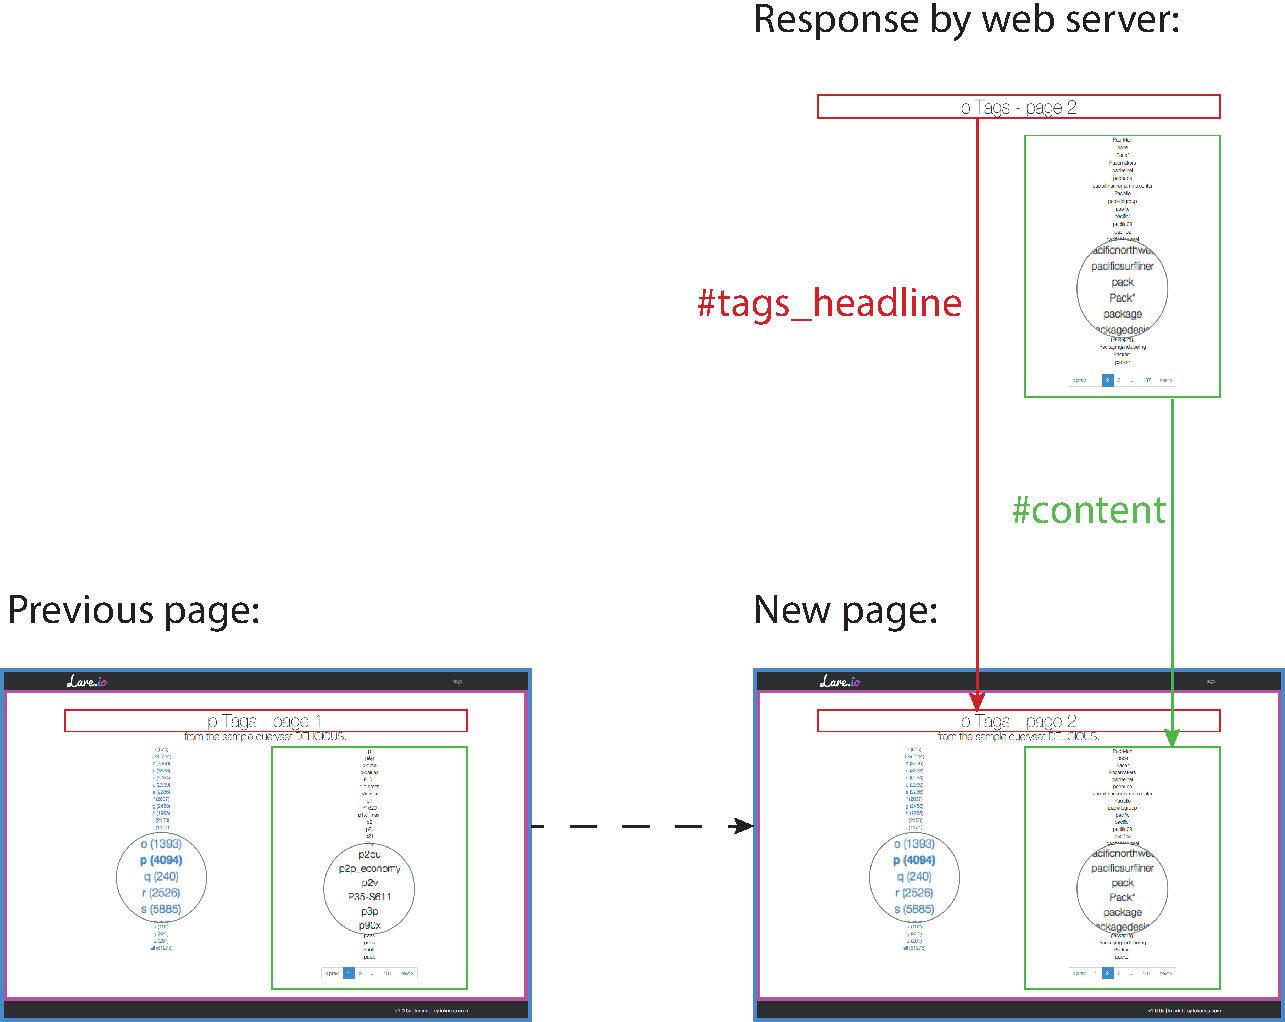
\includegraphics[width=14cm]{images/lare_replacements.pdf}
\caption[lare_replacements]{Content replacements by \lare{}}
\label{fig:lare_replacements}
\end{figure}

\subsection{Concept\label{sec:lare_concept}}

Every \singlePageApplication{} which uses \lare{} has a hierachical namespace structure.
Typically the namespace consists of up to four levels: a site ID, a page ID, a content ID and an inner-content ID.
In our sample web application namespaces like Lare.Tags.P1 are used.
\enquote{Lare} represents the site level, \enquote{Tags} the page and \enquote{P1} the content level.
Every level in the hierarchy has it's counterparts on the \webSite{} as shown in figure \ref{fig:lare_html}.
There is no strict rule where exactly those containers have to be, but a container \emph{A} should not exist in another container \emph{B} if \emph{B} belongs to a namespace level above the one \emph{A} belongs to.
In this case when replacing \emph{B} with other content of the same level it could happen that \emph{A} could not be replaced anymore, because an object with this ID is not in the DOM anymore.
\\
After the \lare{} frontend is initialized it hijacks events like clicks on links and enriches the request with the current page's namespace.
A \lare{} backend plugged into the application analyzes the namespace of the requested page and the one sent in the request.
An earlier interpretation of the \lare{} namespaces like in a \webServer{} plugin for e.g. Apache\footnote{\url{http://httpd.apache.org/}} or Nginx\footnote{\url{http://nginx.org/}} is not possible, because the current request's namespace is set inside the application.
For every hierarchy level it checks if both namespaces match.
If on one level the namespaces differ, the containers according to this level will be responded to the request.
An optimized web application only fetches the data necessary for those containers and renders them afterwards.
The \lare{} frontend retrieves the response, replaces the containers at the \webSite{} and updates the current namespace.

\begin{figure}[H]
\centering
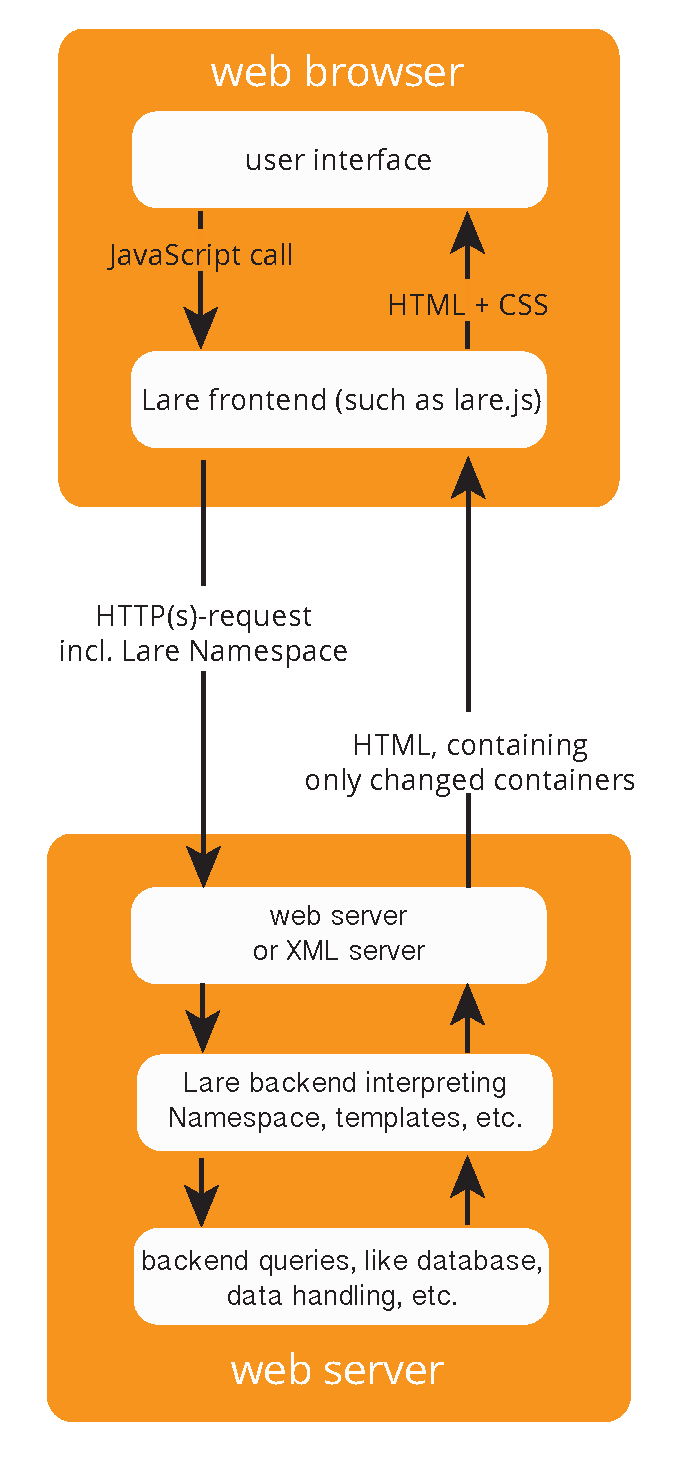
\includegraphics[height=15cm]{images/lare.pdf}
\caption[lare_components]{Components and communication diagram of \lare{}}
\label{fig:lare_components}
\end{figure}


\noindent{}As shown in fig. \ref{fig:lare_components} the rough structure of \lare{} is similar to normal \ajax{} requests shown in fig. \ref{fig:ajax_components}.
The \lare{} frontend, e.g. \lareJS{}, takes the place of the \ajax{} engine.
In addition to \ajax{}, \lare{} has a backend which helps to reduce server load and maps responses to the given namespace.
It can decide which backend queries such as database queries are necessary in the current request.
Additionally it should decide which templates are needed, as \lare{} responses have a different structure than normal HTML documents, which is presented later on.

\subsection{Realization\label{sec:lare_realization}}
To load a page, the first request is a normal \httpRequest{} followed by a JavaScript script initializing the \lare{} frontend module.
This delayed transfer of the frontend is not a problem, as the content can be rendered completely without it.
With this \lare{} follows the \hijax{} pattern, as it fully degrades for usage without JavaScript.
Further requests to the same host are initiated by this module.
The \http{} header of these requests is extended by the namespace of the current \webSite{}.
The web server using a \lare{} backend compares the namespace of the requested resource and the namespace in the \http{} header.
Afterwards it decides which data is needs to be gathered and which template should be used to render those.
\\
The content delivered by the \lare{} backend enriched web server is interpreted by the frontend module and replaces the related containers.
This replacement is implemented using the ID attribute.
Other methods identifying corresponding containers, e.g. X-Path are not as generic in it's position on the page as the ID.
When a container is injected into the Document Object Model(DOM) or the position within a container is changed, the X-Path might not hit the correct container anymore.
For example the X-PATH \emph{//*[@id="page"]/div[2]} will not hit anymore if the previous div gets deleted.
\\
Using the History API makes it possible to update the URL like it would be made by normal requests.
This is realized by the use of the pushState method introduced in the History API.
Back- and forward-buttons and bookmarks in a browser will also behave like they would at normal requests.
\\
The same URL is used by common \httpRequest{}s and \lare{} requests, but the response to the former will be a full \webPage{}, the latter will receive only the changed containers.
Search engines and other crawlers are able to crawl every link they can find and request it as on common \webPage{}s without any deficit.

\subsubsection{\lare{} frontend\label{sec:lare_frontend}}

A \lare{} frontend has, as mentioned before, a few things to be implemented.
The first requirement is the ability to hijack page changes.
This can be implemented by replacing the default event listeners for anchor-tags.
A new event listener has to implement an enrichment of the HTTP header by the namespace using the \enquote{HTTP-X-LARE} key.
On initial requests the current namespace should be served as an attribute of the \emph{<body>} tag called \enquote{data-lare-namespace}.
\lare{} requests serve a new namespace as content of a tag \emph{<pjaxr-namespace>}.
\\
The key feature of \lare{}, dynamic URL changes, have to be implemented after getting the response.
This should be done by using the pushState function.
\\
The key functionality of the \lare{} frontend is the replacement.
A response of a \lare{} request is divided into a \emph{<lare-head>} tag, a \emph{<lare-body>} tag and the \emph{<lare-namespace>} tag.
Elements of the \emph{<lare-head>} should be a new \emph{<title>} tag and \emph{<meta>} tags matching the new content. 
Additionally scripts or styles can be linked in this section when they are needed by the new content.
Tags in the head will be appended, except the title which will be replaced.
\\
The \emph{<lare-body>} tag will contain the new content which should replace existing elements.
The id of every direct child of this tag will be searched on the current \webPage{} and will be replaced if found.
Tags which are part of the response and not found on the current page will be ignored.

\subsubsection{\lare{} backend\label{sec:lare_backend}}

A \lare{} backend should first interpret the \enquote{HTTP-X-LARE} item in the HTTP header.
Every layer of the namespace should have it's own name.
As a default naming convention the layers should have the names \emph{site}, \emph{page}, \emph{content}, \emph{inner\_content} from start to the end.
Per layer a variable should save the matching state.
Those variables have to be accessible by views and controllers to give them the possibility to decide which backend requests should be made and which templates should be used.

\subsubsection{\lare{} templating\label{sec:lare_templating}}

To avoid overhead when using \lare{} a specific templating system is recommended.
\\
A default template for initial requests may be similar to the following:

\begin{minipage}[c]{0.95\linewidth}
\begin{lstlisting}[caption=\_\_base.html, label=lst:example_lare_base_template]
<!Doctype html>
<html>
<head>
  <title></title>
  <script src="lare.min.js"></script>
  ...
</head>
<body data-lare-namespace="{{lare_current_namespace}}">
  
    <div id="site">
      ...
      
      ...
    </div>
  
  
    <div id="additional_lare_includes"></div>
  
</body>
</html>
\end{lstlisting}
\end{minipage}
\\
The only specific code which is necessary for \lare{} to write, is the \emph{data-lare-namespace} attribute at the body tag and the script in the head.
When using a template engine like Twig which can extend templates, \{\% block page \%\} represents a placeholder for where the page specific content will be rendered.
If extensions are not possible, \{\% block page \%\} will be the position where the page specific content would be included.
\\
The \lare{} template could then be formed like this:

\begin{minipage}[c]{0.95\linewidth}
\begin{lstlisting}[caption=\_\_lare.html, label=lst:example_lare_template]
<lare-head>
  <title></title>
  ...
</lare-head>
<lare-body>
  
    
      
    
  
  
  
</lare-body>
<lare-namespace>{{lare_current_namespace}}</lare-namespace>
\end{lstlisting}
\end{minipage}
\\
The <lare-head> tag is the counterpart to the <head> tag, <lare-body> to <body>.
Instead of an attribute in the <lare-body> tag, the namespace will be delivered in the <lare-namespace> tag.
\\
The tags page in our sample web application consists of two templates.
On the one hand the character specific tags.html, seen in listing \ref{lst:tags_template}, which belongs to the third level namespace.
On the other hand there is \_\_tags\_base.html, visible in listing \ref{lst:tags_base_template}, which needs to get rendered only when entering the tags section and belongs to the second level namespace.

\begin{minipage}[c]{0.95\linewidth}
\begin{lstlisting}[caption=tags.html, label=lst:tags_template]


  <div id="content">
    ... // Tags list and pagination
  </div>


  <h1 id="tags_headline">
    {{ current_char }} Tags - page {{ current_page }}
  </h1>

\end{lstlisting}
\end{minipage}


\begin{minipage}[c]{0.95\linewidth}
\begin{lstlisting}[caption=\_\_tags\_base.html, label=lst:tags_base_template]


<div id="page">
  ...
  <h1 id="tags_headline">
    {{ current_char }} Tags - page {{ current_page }}
  </h1>
  ... // Character list
  
  ...
</div>

\end{lstlisting}
\end{minipage}

\noindent{}When e.g. navigating from the first page of P tags to the second page, the first two namespaces match, the third differs.
The third level belongs to \{\% block content \%\} in which the container with the id \enquote{content} is placed.
Additionally the container with the id \enquote{tags\_headline} is required to be replaced. As it is not a sibling of the content part it can be replaced in the \enquote{additional\_lare\_includes} block.
The response in this case is shown in listing \ref{lst:lare_response}.

\begin{minipage}[c]{0.95\linewidth}
\begin{lstlisting}[caption=Example Lare Response, label=lst:lare_response]
<lare-body>
  <div id="content">
    ... // Tags list and Pagination
  </div>
  <div id="tags_headline">
    P Tags - page 2
  </div>
</lare-body>
<lare-namespace>Lare.Tags.P2</lare-namespace>
\end{lstlisting}
\end{minipage}

\noindent{}Both necessary containers are rendered.
The content div is rendered, because it is defined in the content block and the tags\_headline div is defined inside the additional\_lare\_includes block.
\\
This block is intended to update content which is not inside the current level's container, in this case tags\_headline is inside the site level of the \enquote{Tags} namespace.


\newpage{}

\section{Implementation}

\todo{decisions Lare Object}
We decided to implement the \lare{} backend in two parts.
Considering the MVC pattern we have all logic in one object, in this case the Lare object.
It is a singleton in the request scope.
When receiving a request the server creates it and analyzes if the current request is a \lare{} request and checks if there is a namespace.


\subsection{\phpLare{}}
\phpLare{} is a general \lare{} backend to used in PHP.
It builds the base of every other Lare module in PHP, especially for template engines.

\lare{} is a implemented as a request-scoped Singleton.
In PHP a singleton is implemented as a class, which provides only static methods and static attributes.

\subsubsection{API}

When including the Lare.php automatically a Singleton named Lare will be created.
\begin{itemize}
\item Lare::is\_enabled()

Returns true if the current request is a Lare request, otherwise false.
\item Lare::set\_current\_namespace(\$namespace)

Sets the namespace of the current request to \$namespace.
\item Lare::get\_current\_namespace()

Returns the namespace of the current request.
\item Lare::get\_matching(\$extension\_namespace = null)

\$extension\_namespace is an optional paramenter, to check the matching to a given namespace. If \$extension\_namespace is not given, the matching will be done against the namespace of the current request.

Returns the most specific matching namespace level.
\item Lare::matches(\$extension\_namespace = null)

\$extension\_namespace is an optional paramenter, to check the matching to a given namespace. If \$extension\_namespace is not given, the matching will be done against the namespace of the current request.

Returns true if the whole namespace is matching, otherwise false.
\end{itemize}
    
\subsection{\twigLare{}}
Twig-Lare brings Lare functionality to the template engine Twig\footnote{http://twig.sensiolabs.org/}.
Twig is used by Symfony, a framework which is used in e.g. Drupal 8, eZPublish, phpBB and Sylius.

Twig-Lare is a implemented as a Twig extension.
It consists of a TwigTokenParser, a anonymous TwigSimpleFunction and a global variable.
The TwigTokenParser Twig\_Lare\_TokenParser\_LareExtends is the heart of the extension.
It provides the possibility to use the tag \{\% lare\_extends \%\} in the way it may be used in django.
To prevent multiple extend tags, including the default twig tag \emph{\{\% extends \%\}} it throws a Error if either the default tag or \{\% lare\_extends \%\} was already used.
Additionally we ensure that it is not called inside a block tag.

\begin{minipage}[c]{0.95\linewidth}
\begin{lstlisting}


  <div id="page">
    ...
  </div>

{{ current_lare_namespace }}
\end{lstlisting}
\end{minipage}

The example above shows the usage of this tag.
When the current namespace is not inside Lare.Namespace it extends to the \:\:\_\_base.twig template because the second namespace does not match then.
But when the current namespace is \emph{Lare.Namespace}, then it extends \:\:\_\_lare.twig.

As the namespace matching occurs on the second level in this example, the overriden block should be the second, with the naming in this thesis \emph{page}.
Inside this block a <div> container with the according ID has to be placed.

\subsubsection{API}

\begin{itemize}
\item \{\% lare\_extends \$default\_template \%\}

Extends \$default\_template like the original \{\% extends \$default\_template \%\}.
\item \{\% lare\_extends \$default\_template \$lare\_namespace \%\}

Extends ::\_\_lare.html if \$lare\_namespace is matching, otherwise it extends \$default\_template.
\item \{\% lare\_extends \$default\_template \$lare\_template \$lare\_namespace \%\}

Extends \$lare\_template if \$lare\_namespace is matching, otherwise it extends \$default\_template.
\end{itemize}


\subsection{\djangoLare{}}

\djangoLare{} was the first backend of \lare{}.
It was introduced as a single object containing logic and template tools.
After implementing \phpLare{} we decided to change the structure of the django backend towards the new segmentation.

Similar to the combination of \phpLare{} and \twigLare{}, \djangoLare{} consists of a Lare object as in the PHP backend and implements the same templating tools as the Twig extension.
Still as one package it is available via \emph{pip install django-lare} command.

\subsection{\lareJS{}}
\lareJS{}, as successor of jquery-pjaxr, is the frontend engine for \lare{}, using AJAX to communicate to the server.
jQuery-pjaxr was introduced as an extended version of jquery-pjax, allowing to replace multiple containers with one request, instead of only one.
Matching by the ID of an container it was not the job of the frontend to define which container should be replaced, but the backend with giving the correct IDs.

Introducing \lareJS{} achieved the ability differ the current page via namespaces.
\todo{describe \lareJS{}}


\subsection{concluding remarks}


\newpage{}

\section{Evaluation}
\lare{} is tested based on a sample web application.
It provides different type of sites which are designed to perform the different aspects of this evaluation.

To evaluate \lare{} we first test it's functionality.
We check if the desired content is delivered and if \lare{} is actually performing like expected.

It is not easy to test \ajax{} \webApplication{}s.
As seen in \footnote{http://selab.fbk.eu/tonella/papers/wqvv2007.pdf} there is a lack of good testing tools, especially when it comes to white-box testing.
For black-box testing a good tool is selenium.

In \footnote{http://selab.fbk.eu/tonella/papers/icst2008.pdf} the same authors introduce a new automated testing technique, again based on selenium.

As to evaluate \lare{} there is no need to actually test the whole application, but only to check whether \lare{} works, selenium in our case is sufficient.

We make specific requests and want an specific answer of it.
Especially we want to have the same content rendered through \lare{} as through normal \httpRequest{}s.

Selenium additionally makes it possible to use different WebDrivers, in this thesis FireFox and Chrome are used.
This is important because of the different implementations of browsers' features.

To test the performance, we will use two technologies.
\footnote{http://swerl.tudelft.nl/twiki/pub/Main/TechnicalReports/TUD-SERG-2008-009.pdf}.
First of all curl-based tests will be done.
Those tests will focus on the first response, containing the markup.
This will show how \lare{} influences the webserver.

Additionially the webapp will be benchmarked by using the Chrome Network Tools.
This method provides the possiblity to check whether further requests for scripts, images, etc. are influenced.
The Chrome Network Tools will show the actual load time the user has to wait for, until the whole page is loaded.

To make the tests as representive as possible, caching in every dimension will be enabled and disabled to see whether it influences the results or not.
As I use Mysql as database I will enable and disable the query caching.
Twig, the template engine allows caching, which will be enabled and disabled as well.
Additionally all tests are performed on a local machine and a remote server, to see whether the latency takes effect in the performance of \lare{}.

We will not do load tests with multiple users as the amount of concurrent users should be up to 10000 to be representative\footnote{http://swerl.tudelft.nl/twiki/pub/Main/TechnicalReports/TUD-SERG-2008-009.pdf}.
In this thesis this we will not be able to do that, due to the lack of a Supercomputer such as used in \footnote{http://swerl.tudelft.nl/twiki/pub/Main/TechnicalReports/TUD-SERG-2008-009.pdf}.

We will distinguish between static pages without database queries and dynamic pages which have those.
Every page relevant for the test will be requested in different modes.
First of all every site will be requested normally.
After that it will be requested with \lare{} enabled.
As \lare{} should only influence subsequent requests, every page will be tested with \http{} headers from different sources, imitating those requests.

%As one traditional testing model, we will evaluate the \pjaxr{} sample application via blackbox tests.
%Testing \ajax{} is not trivial due to multiple programming- and markup-languages influencing it. 
%One possibility to test web applications, as suggested in \cite{bib:lundmark11}, is Selenium\footnote{http://www.seleniumhq.org/}.
%With this tool it is possible to generate automated tests for web applications.
%
%To evaluate whether the application is crawlable or not is an important criteria whether \pjaxr{} fulfills it goals.
%Finding all the content delivered in all different URLs in the sitemap should be the target to acquire.
%The crawled content should be similar to a non-dynamic HTML file, defined for every URL.
%Content which is not directly provided via an URL but asynchronously, like via an autocompletion, should not be relevant.
%
%One way to crawl \ajax{} web applications, recommended in \cite{bib:crawljax_tweb12} is to use Crawljax\footnote{http://crawljax.com/}. 
%It explores \ajax{}-based web applications by following every link recursively and saving the associated content. In this thesis the three endpoints of the sample project will be crawled by Crawljax to see whether all endpoints provide the same content or not.
%
%Another way to evaluate whether \pjaxr{} fulfils its goals, is testing if the Googlebot\footnote{http://google.com/bot.html} will discover all the content provided.
%Again, all three endpoints will be tested to check, if all data is found by this technique.
%While Crawljax is intended to find not easily accessible content, Googlebot is intended to find content, matching design patterns\footnote{https://developers.google.com/webmasters/ajax-crawling/} by Google. This fact makes it more challenging for \pjaxr{}, not implementing these, to have good results in this test.


\subsection{Sample web application}

The sample web application used to test \lare{} in this thesis is implemented in PHP.
To implement \lare{} we used \lareJS{} in the frontend, \twigLare{} and \phpLare{} for the backend.

We use the MVC design pattern, but with a slightly different naming.
For web applications it is common to use the name \emph{template} for what is called view in the MVC.
As "controller" is not a common name PHP web applications as well, we use the phrase \emph{view} for those.
With this we follow the naming of django\footnote{https://docs.djangoproject.com/en/1.8/faq/general/\#django-appears-to-be-a-mvc-framework-but-you-call-the-controller-the-view-and-the-view-the-template-how-come-you-don-t-use-the-standard-names}.

Instead of using models for this benchmark evaluation, we are using raw SQL queries to ensure the same queries are made every time.
Nevertheless it is prepared to inherit from the BaseModel class to be create models for later presentation purposes.

The sample web application consists of 2 static pages \emph{/home/} and \emph{/imprint/}.

To demonstrate dynamic \WebPage{}s we used the Delicious Dataset\footnote{http://fabianabel.de/data/mypes-www2010.html}.
This is available under \emph{/tags/}.

On the left side is a list to sub pages where the tags are categorized by it's starting character.
Per alphabetic character one of those pages exists, additionally one page for tags starting with numbers and one starting with non alphanumeric characters.
Behind each \emph{category} the count of tags in this category is displayed.
This list is available on every sub page under the \emph{/tags/} url.

On the right side a paginated list of all distinct tags in the current category is shown.
It is sorted alphabetically and 30 tags per page are displayed.

We are using the namespaces like shown in tab. \ref{tab:sampleapp_namespaces}.

\begin{table}[h]
\centering
\begin{tabular}{llll}
	\hline
	\textbf{URL} & \textbf{Site} & \textbf{Page} & \textbf{Content} \\
	\hline
	/ & Lare & Home &  \\
	/imprint/ & Lare & Imprint &  \\
	/tags/ & Lare & Tags & all \\
	/tags/a/ & Lare & Tags & a \\
	/tags/.../ & Lare & Tags & ... \\
	\hline
\end{tabular}
\caption{Namespaces of the sample web application}
\label{tab:sampleapp_namespaces}
\end{table}


\subsection{Tests}

To test the performance of \lare{} a few different types of requests are needed to benchmark.
The reference level will be a normal \httpRequest{} to each \webPage{}.

The tested pages are available at the URLs:

\begin{itemize}
\item /
\item /imprint/
\item /tags/p/
\item /tags/p/2/
\end{itemize}

Additionally the \webPage{}s will be requested via \lare{}.
To achieve this at curl we extend the request's header with the corresponding \emph{HTTP-X-LARE} namespace.

With Selenium we will later test the pages with real web browsers to get results which are closer to reality.
The tested page to page requests are:

\begin{itemize}
  \item Self:
    \begin{itemize}
      \item / to /
      \item /imprint/ to /imprint/
      \item /tags/p/ to /tags/p/
      \item /tags/p/2/ to /tags/p/2/
    \end{itemize}
  \item Static page matching Site-Namespace:
    \begin{itemize}
      \item / to /imprint/
      \item /imprint to /
    \end{itemize}
  \item Dynamic page matching Site-Namespace:
    \begin{itemize}
      \item / to /tags/p/
      \item /imprint/ to /tags/p/
    \end{itemize}
  \item Dynamic page to static page:
    \begin{itemize}
      \item /tags/p/ to /
      \item /tags/p/2/ to /
      \item /tags/p/ to /imprint/
      \item /tags/p/2/ to /imprint/
    \end{itemize}
  \item Dynamic page matching Page-Namespace:
    \begin{itemize}
      \item /tags/p/ to /tags/p/2/
      \item /tags/p/2/ to /tags/p/
    \end{itemize}
\end{itemize}

\subsection{Curl\label{curl}}

We are using curl to test the plain load times of the initial request of normal \httpRequest{}s and \lare{} requests.
Those curl requests do not include additional data like images, scripts and stylesheets, just the plain HTML.

The bash script \enquote{curl\_tests.sh} provides the functionality to run those curl tests.
To use it run 
\enquote{/.../evaluation/curl/curl\_tests.sh URL MAX\_RUNS LARE\_NAMESPACE CACERT}.

URL dedicates where the web application is available, e.g. \emph{http://lare.iekadou.com}, MAX\_RUNS defines how many curl requests per page should be made.
LARE\_NAMEPSACE defines the namespace, which should be used when testing the \lare{} requests, e.g. Lare.Tags.p.
CACERT is the only optional paremeter, which should only be set when requesting an SSL server. It then should be the path to the CACERT file.


To test all relevant sites we defined a variable PAGES inside the script, containing URLs \emph{/}, \emph{/imprint/}, \emph{/tags/p/} and \emph{/tags/p/2/}.
For each page of those we make a normal request, followed by a \lare{} request, with the namespace defined in LARE\_NAMESPACE. 
To get better test results we repeat those two requests \emph{MAX\_RUN} times. The output represents then the load times needed in seconds.

For the results in this thesis, markes as local, we use a Macbook Pro Retina Early 2013 (2,7 GHz, 16GB Ram).
As web server we are running an Apache via Mamp Pro 3.1 for Mac OSX with PHP 5.3.6.
As database server we are using MySQL in version 5.5.42.

When running the benchmarks on an external server we are using a virtual server running OS: Ubuntu 12.04.5 LTS.
It has a Intel(R) Xeon(R)CPU E5520, 4 GB ram, PSA version 11.5.30, Mysql version 5.5.41 and php version 5.3.10.

Additionally we test every request with database caching (DBC) enabled, disabled and template caching(TC) enabled and disabled.

\subsubsection{Results}

You can see the full results of our benchmarks in tables \ref{tab:curl_results_local} and \ref{tab:curl_results_external}.

First we will take a look at the results of the local tests.

Those tests show that the load times of \lare{} requests of static pages in general are quite the same then on normal \httpRequest{}s.
\lare{} does not seem to have a huge effect on static pages without a lot of heavy operations like backend queries. It makes the responses a bit smaller, but no logical operations can be avoided.

Template caching has not a big effect on the difference between \lare{} and normal requests, but the absolute load times get a bit down.
Database caching has not even on the absolute times an effect at those static pages, because no backend queries are made.

When requesting a dynamic page and sending the namespace of a static page like in our tests \enquote{Lare.Tags.Imprint} the results of \lare{} are still similar to normal requests.
This can be explained by the fact that almost the whole page needs to be changed, including every database query.

The results on dynamic pages with a related namespace, in our case \enquote{Lare.Tags.p} differ a lot.
When database caching is enabled the load times of \lare{} are around 90\% with template caching enabled and about 80\% of the normal load times with disabled template caching.

Without database caching this these times they are \textbf{7\%} with template caching and \textbf{10\%} without.

Those improvemnts are caused by the amount of database queries that can be avoided. This also explains the differences between enabled and disabled database caching settings.

When we take a look at the external tests we can see the same pattern.
The effect of \lare{} on dynamic pages is a bit smaller.
Wihtout database caching they are about \textbf{12\%} with template caching and \textbf{16\%} without.

Why does it have not this huge effect anymore?

This can be explained with the latency.
In our tests it was 40ms.
\httpRequest{}s need two Round Trip Times, or four times the latency for connection establishment.
When we substract those 160ms from the normal and the \lare{} requests we see ratios similar to the local tests.

In general we can say, that \lare{} has more effect the more time of backend logic like database queries can be avoided.

\newpage{}

\begin{center}
\begin{longtable}{llllll}
	\hline
	\textbf{URL} & \textbf{Normal loadtime} & \textbf{\lare{} loadtime} & \textbf{Namespace} & \textbf{TC} & \textbf{DBC} \\
	\hline
	/ & 0.03740 & 0.03600 (96,26\%) & Lare.Tags.p & + & + \\
	/imprint/ & 0.03590 & 0.03620 (100,84\%) & Lare.Tags.p & + & + \\
	/tags/p/ & 0.03950 & 0.03480 (88,10\%) & Lare.Tags.p & + & + \\
	/tags/p/2/ & 0.03940 & 0.03550 (90,10\%) & Lare.Tags.p & + & + \\
	\hline
	/ & 0.03370 & 0.03610 (107,12\%) & Lare.Tags.Imprint & + & + \\
	/imprint/ & 0.03570 & 0.03450 (96,64\%) & Lare.Tags.Imprint & + & + \\
	/tags/p/ & 0.03910 & 0.04080 (104,36\%) & Lare.Tags.Imprint & + & + \\
	/tags/p/2/ & 0.04040 & 0.03960 (98,02\%) & Lare.Tags.Imprint & + & + \\
	\hline
	\hline
	/ & 0.03400 & 0.03380 (99,41\%) & Lare.Tags.p & + & - \\
	/imprint/ & 0.03430 & 0.03480 (101,46\%) & Lare.Tags.p & + & - \\
	\textbf{/tags/p/} & \textbf{1.02180} & \textbf{0.07230 (7,08\%)} & \textbf{Lare.Tags.p} & \textbf{+} & \textbf{-}\\
	/tags/p/2/ & 1.03130 & 0.07310 (7,09\%) & Lare.Tags.p & + & - \\
	\hline
	/ & 0.03440 & 0.03650 (106,10\%) & Lare.Tags.Imprint & + & - \\
	/imprint/ & 0.03540 & 0.03480 (98,31\%) & Lare.Tags.Imprint & + & - \\
	/tags/p/ & 1.02390 & 1.04130 (101,70\%) & Lare.Tags.Imprint & + & - \\
    \textbf{/tags/p/2/} & \textbf{1.03440} & \textbf{1.04980 (101,49\%)} & \textbf{Lare.Tags.Imprint} & \textbf{+} & \textbf{-}\\
    \hline
	\hline
	/ & 0.07210 & 0.06660 (92,37\%) & Lare.Tags.p & - & - \\
	/imprint/ & 0.06690 & 0.06410 (95,81\%) & Lare.Tags.p & - & - \\
	/tags/p/ & 1.08420 & 0.10720 (9,89\%) & Lare.Tags.p & - & - \\
    \textbf{/tags/p/2/} & \textbf{1.09660} & \textbf{0.10900 (9,94\%)} & \textbf{Lare.Tags.p} & \textbf{-} & \textbf{-}\\
    \hline
	/ & 0.06920 & 0.06860 (99,13\%) & Lare.Tags.Imprint & - & - \\
	/imprint/ & 0.06840 & 0.06520 (95,32\%) & Lare.Tags.Imprint & - & - \\
	/tags/p/ & 1.09020 & 1.09620 (100,55\%) & Lare.Tags.Imprint & - & - \\
	/tags/p/2/ & 1.09000 & 1.07740 (98,84\%) & Lare.Tags.Imprint & - & - \\
	\hline
	\hline
	/ & 0.07070 & 0.06630 (93,78\%) & Lare.Tags.p & - & + \\
	/imprint/ & 0.06710 & 0.06510 (97,02\%) & Lare.Tags.p & - & + \\
	/tags/p/ & 0.08440 & 0.06990 (82,82\%) & Lare.Tags.p & - & + \\
	/tags/p/2/ & 0.08550 & 0.06930 (81,05\%) & Lare.Tags.p & - & + \\
	\hline
	/ & 0.07010 & 0.06790 (96,86\%) & Lare.Tags.Imprint & - & + \\
	/imprint/ & 0.06770 & 0.06510 (96,16\%) & Lare.Tags.Imprint & - & + \\
	/tags/p/ & 0.08540 & 0.08230 (96,37\%) & Lare.Tags.Imprint & - & + \\
	\textbf{/tags/p/2/} & \textbf{0.08390} & \textbf{0.08220 (97,97\%)} & \textbf{Lare.Tags.Imprint} & \textbf{-} & \textbf{+} \\
	\hline
\caption{Curl results on a local machine}
\label{tab:curl_results_local}
\end{longtable}
\end{center}



\begin{center}
\begin{longtable}{llllll}
	\hline
	\textbf{URL} & \textbf{Normal loadtime} & \textbf{\lare{} loadtime} & \textbf{Namespace} & \textbf{TC} & \textbf{DBC} \\
	\hline
	/ & 0.16520 & 0.14070 (85,17\%) & Lare.Tags.p & + & + \\
	/imprint/ & 0.14360 & 0.12850 (89,48\%) & Lare.Tags.p & + & + \\
	/tags/p/ & 0.15420 & 0.13180 (85,47\%) & Lare.Tags.p & + & + \\
	/tags/p/2/ & 0.14610 & 0.14200 (97,19\%) & Lare.Tags.p & + & + \\
	\hline
	/ & 0.14050 & 0.13350 (95,02\%) & Lare.Tags.Imprint & + & + \\
	/imprint/ & 0.13690 & 0.13630 (99,56\%) & Lare.Tags.Imprint & + & + \\
	/tags/p/ & 0.14470 & 0.14170 (97,93\%) & Lare.Tags.Imprint & + & + \\
	/tags/p/2/ & 0.14230 & 0.13310 (93,53\%) & Lare.Tags.Imprint & + & + \\
	\hline
	\hline
	/ & 0.14860 & 0.14580 (98,11\%) & Lare.Tags.p & + & - \\
	/imprint/ & 0.14990 & 0.13830 (92,66\%) & Lare.Tags.p & + & - \\
	\textbf{/tags/p/} & \textbf{1.55500} & \textbf{0.19070 (12,26\%)} & \textbf{Lare.Tags.p} & \textbf{+} & \textbf{-} \\
	/tags/p/2/ & 1.52150 & 0.19600 (12,88\%) & Lare.Tags.p & + & - \\
	\hline
	/ & 0.14160 & 0.14080 (99,44\%) & Lare.Tags.Imprint & + & - \\
	/imprint/ & 0.14300 & 0.13790 (96,43\%) & Lare.Tags.Imprint & + & - \\
	/tags/p/ & 1.50930 & 1.54400 (102,30\%) & Lare.Tags.Imprint & + & - \\
	\textbf{/tags/p/2/} & \textbf{1.51030} & \textbf{1.56460 (103,59\%)} & \textbf{Lare.Tags.Imprint} & \textbf{+} & \textbf{-} \\
	\hline
	\hline
	/ & 0.20450 & 0.18600 (90,95\%) & Lare.Tags.p & - & - \\
	/imprint/ & 0.20350 & 0.18130 (89,09\%) & Lare.Tags.p & - & - \\
	/tags/p/ & 1.64180 & 0.30550 (18,61\%) & Lare.Tags.p & - & - \\
	\textbf{/tags/p/2/} & \textbf{1.65950} & \textbf{0.24830 (14,96\%)} & \textbf{Lare.Tags.p} & \textbf{-} & \textbf{-} \\
	\hline
	/ & 0.20390 & 0.19800 (97,11\%) & Lare.Tags.Imprint & - & - \\
	/imprint/ & 0.20440 & 0.18360 (89,82\%) & Lare.Tags.Imprint & - & - \\
	/tags/p/ & 1.64260 & 1.62680 (99,04\%) & Lare.Tags.Imprint & - & - \\
	/tags/p/2/ & 1.63810 & 1.67440 (102,22\%) & Lare.Tags.Imprint & - & - \\
	\hline
	\hline
	/ & 0.20940 & 0.20020 (95,61\%) & Lare.Tags.p & - & + \\
	/imprint/ & 0.20300 & 0.19040 (93,79\%) & Lare.Tags.p & - & + \\
	/tags/p/ & 0.22250 & 0.20760 (93,30\%) & Lare.Tags.p & - & + \\
	/tags/p/2/ & 0.20940 & 0.20160 (96,28\%) & Lare.Tags.p & - & + \\
	\hline
	/ & 0.20800 & 0.20500 (98,56\%) & Lare.Tags.Imprint & - & + \\
	/imprint/ & 0.19970 & 0.19480 (97,55\%) & Lare.Tags.Imprint & - & + \\
	/tags/p/ & 0.21420 & 0.20200 (94,30\%) & Lare.Tags.Imprint & - & + \\
	\textbf{/tags/p/2/} & \textbf{0.21630} & \textbf{0.22510 (104,07\%)} & \textbf{Lare.Tags.Imprint} & \textbf{-} & \textbf{+} \\
	\hline
\caption{Curl results on a external machine}
\label{tab:curl_results_external}
\end{longtable}
\end{center}

\subsection{Selenium}

To benchmark full page loads including all resources we are using selenium.
This \emph{record and play} tool builds an interface for a usage of multiple webdrivers.
Those webdrivers are provided by most modern browsers like Chrome and Firefox.
For the results in this thesis we used the Firefox webdriver.

We request a page via a normal \httpRequest{} first.
Afterwards we request the same page again via \lare{}.
We are using a lot of different page to page requests, to see where \lare{} has a bigger or smaller effect on the load times.

Like in \ref{curl} we test every page on a local server and an external webserver and we disabled and enable database and template caching.

\subsubsection{Results}

The results of the selenium webdriver tests are different to the ones made with curl.

We first will take a look at the local tests again.
Other than in the curl test results we see a huge effect of \lare{} even on the static pages.
An average \lare{} load time of about 35\% with disabled template caching and 9\% with enabled template caching of the normal load time can be seen here.   2
Other than on a normal request, the browser does not need to load the resources like images, scripts and styles.
This means \lare{} requests often only need one request to make a page change.
A normal requests needs to load, or at least compare, about 9 resources for the same action.

Again requesting a static page does not show any changes when it comes to database caching.

When it comes to dynamic pages we have to take a more detailed look to the requests.
Requesting a dynamic page from another \lare{} namespace with disabled database caching takes almost the same time like a normal request.
This is because the same backend requests need to be done.
Those uncached database requests take as we can see in table \ref{tab:curl_results_local} the majority of time.

With disabled caching in the database and in a related namespace instead, \lare{} has a huge effect.
Enabled template caching improving the load times from 5\% with a disabled template caching to 3,5\%.

When requesting the same pages with enabled database caching we see a \lare{} load time of about 16\% with unrelated namespaces.
Related namespaces in the same configuration lead to values of about 10\%.

Enabled template caching lower the load times of the normal and \lare{} requests, but not of the resources.
This makes \lare{} more effective, because the load times relative to the normal requests incl. all resources decrease.


\begin{center}
\begin{longtable}{llllll}
	\hline
	\textbf{From} & \textbf{To} & \textbf{Normal loadtime} & \textbf{\lare{} loadtime} & \textbf{TC} & \textbf{DBC} \\
	\hline
	/tags/p/ & /tags/p/2/ & 60.0648983ms & 7.3076173ms (12.17\%) & + & + \\
	/tags/p/2/ & /tags/p/ & 51.5302378ms & 5.7457083ms (11.15\%) & + & + \\
	\hline
	/tags/p/ & / & 58.0190003ms & 5.2543307ms (9.06\%) & + & + \\
	/tags/p/2/ & / & 45.1883941ms & 4.159042ms (9.20\%) & + & + \\
	/tags/p/ & /imprint/ & 46.8359346ms & 4.3459044ms (9.28\%) & + & + \\
	/tags/p/2/ & /imprint/ & 47.1970978ms & 4.2372439ms (8.98\%) & + & + \\
	\hline
	/ & / & 56.6017328ms & 5.4929997ms (9.70\%) & + & + \\
	/imprint/ & /imprint/ & 43.3243723ms & 4.1624412ms (76.67\%) & + & + \\
	/tags/p/ & /tags/p/ & 54.4607062ms & 5.5379726ms (10.17\%) & + & + \\
	/tags/p/2/ & /tags/p/2/ & 52.5258287ms & 5.7707781ms (10.99\%) & + & + \\
	\hline
	/ & /tags/p/ & 66.8794388ms & 10.4380685ms (15.61\%) & + & + \\
	/imprint/ & /tags/p/ & 52.089504ms & 9.1059678ms (17.48\%) & + & + \\
	\hline
	/ & /imprint/ & 57.6817111ms & 5.884066ms (10.20\%) & + & + \\
	/imprint/ & / & 45.9628159ms & 4.6333061ms (10.08\%) & + & + \\
	\hline
	\hline
	/tags/p/ & /tags/p/2/ & 1243.4891679ms & 46.5173918ms (3.74\%) & + & - \\
	/tags/p/2/ & /tags/p/ & 1236.3124832ms & 43.4368424ms (3.51\%) & + & - \\
	\hline
	/tags/p/ & / & 53.4060902ms & 5.1304958ms (9.61\%) & + & - \\
	/tags/p/2/ & / & 45.4183183ms & 4.206772ms (9.26\%) & + & - \\
	/tags/p/ & /imprint/ & 46.2665835ms & 4.175386ms (9.02\%) & + & - \\
	/tags/p/2/ & /imprint/ & 46.0661066ms & 4.2264232ms (9.17\%) & + & - \\
	\hline
	/ & / & 53.5617939ms & 5.4352539ms (10.15\%) & + & - \\
	/imprint/ & /imprint/ & 45.0215085ms & 4.4406ms (65.68\%) & + & - \\
	/tags/p/ & /tags/p/ & 1234.5362779ms & 44.369364ms (3.59\%) & + & - \\
	/tags/p/2/ & /tags/p/2/ & 1235.7906042ms & 45.1390014ms (3.65\%) & + & - \\
	\hline
	/ & /tags/p/ & 1246.2746233ms & 1197.6706971ms (96.10\%) & + & - \\
	/imprint/ & /tags/p/ & 1231.1385665ms & 1191.9845789ms (96.82\%) & + & - \\
	\hline
	/ & /imprint/ & 49.8334108ms & 6.1112746ms (12.26\%) & + & - \\
	/imprint/ & / & 44.540915ms & 4.2382487ms (9.52\%) & + & - \\
	\hline
	\hline
	/tags/p/ & /tags/p/2/ & 1281.1725193ms & 69.312793ms (5.41\%) & - & - \\
	/tags/p/2/ & /tags/p/ & 1271.3418256ms & 67.1285484ms (5.28\%) & - & - \\
	\hline
	/tags/p/ & / & 81.102332ms & 27.2707205ms (33.63\%) & - & - \\
	/tags/p/2/ & / & 69.681426ms & 25.9004252ms (37.17\%) & - & - \\
	/tags/p/ & /imprint/ & 68.4034544ms & 24.2320953ms (35.43\%) & - & - \\
	/tags/p/2/ & /imprint/ & 66.3318697ms & 23.254195ms (35.06\%) & - & - \\
	\hline
	/ & / & 80.4801214ms & 27.0665394ms (33.63\%) & - & - \\
	/imprint/ & /imprint/ & 66.282428ms & 23.5402204ms (35.52\%) & - & - \\
	/tags/p/ & /tags/p/ & 1277.0515153ms & 67.8621459ms (5.31\%) & - & - \\
	/tags/p/2/ & /tags/p/2/ & 1266.6883795ms & 68.0796981ms (5.37\%) & - & - \\
	\hline
	/ & /tags/p/ & 1274.8229527ms & 1224.9995695ms (96.09\%) & - & - \\
	/imprint/ & /tags/p/ & 1273.1817246ms & 1221.7685327ms (95.96\%) & - & - \\
	\hline
	/ & /imprint/ & 71.5289704ms & 25.8452978ms (36.13\%) & - & - \\
	/imprint/ & / & 70.3443044ms & 26.8150602ms (38.12\%) & - & - \\
	\hline
	\hline
	/tags/p/ & /tags/p/2/ & 96.6278896ms & 31.5540318ms (32.66\%) & - & + \\
	/tags/p/2/ & /tags/p/ & 84.6051469ms & 29.4296049ms (34.78\%) & - & + \\
	\hline
	/tags/p/ & / & 78.0617908ms & 28.0351468ms (35.91\%) & - & + \\
	/tags/p/2/ & / & 70.2056237ms & 26.3221693ms (37.49\%) & - & + \\
	/tags/p/ & /imprint/ & 66.3406013ms & 23.5038ms (35.43\%) & - & + \\
	/tags/p/2/ & /imprint/ & 67.9293146ms & 23.1398233ms (34.06\%) & - & + \\
	\hline
	/ & / & 79.6650023ms & 27.2197206ms (34.17\%) & - & + \\
	/imprint/ & /imprint/ & 65.1834701ms & 23.0573013ms (35.37\%) & - & + \\
	/tags/p/ & /tags/p/ & 89.4712661ms & 29.4440881ms (32.91\%) & - & + \\
	/tags/p/2/ & /tags/p/2/ & 86.7669023ms & 30.3473338ms (34.98\%) & - & + \\
	\hline
	/ & /tags/p/ & 101.7855178ms & 43.100569ms (42.34\%) & - & + \\
	/imprint/ & /tags/p/ & 84.2801923ms & 42.5754955ms (50.52\%) & - & + \\
	\hline
	/ & /imprint/ & 70.6183847ms & 25.6731125ms (36.35\%) & - & + \\
	/imprint/ & / & 69.7824729ms & 25.9579276ms (37.20\%) & - & + \\
	\hline
\caption{Selenium benchmark results on a local machine}
\label{tab:selenium_benchmark_results_local}
\end{longtable}
\end{center}

\newpage{}

\begin{center}
\begin{longtable}{llllll}
	\hline
	\textbf{From} & \textbf{To} & \textbf{Normal loadtime} & \textbf{\lare{} loadtime} & \textbf{TC} & \textbf{DBC} \\
	\hline
	/tags/p/ & /tags/p/2/ & 378.7378772ms & 100.0062951ms (26.41\%) & + & + \\
	/tags/p/2/ & /tags/p/ & 149.1767846ms & 100.5256257ms (67.39\%) & + & + \\
	\hline
	/tags/p/ & / & 177.8015667ms & 101.0766767ms (56.86\%) & + & + \\
	/tags/p/2/ & / & 145.9762462ms & 100.3458274ms (68.74\%) & + & + \\
	/tags/p/ & /imprint/ & 145.1269058ms & 99.0440198ms (68.25\%) & + & + \\
	/tags/p/2/ & /imprint/ & 143.6989026ms & 96.5441573ms (67.19\%) & + & + \\
	\hline
	/ & / & 184.0143055ms & 96.8061586ms (52.61\%) & + & + \\
	/imprint/ & /imprint/ & 146.1839403ms & 102.3730996ms (70.03\%) & + & + \\
	/tags/p/ & /tags/p/ & 158.4086978ms & 96.0358653ms (60.63\%) & + & + \\
	/tags/p/2/ & /tags/p/2/ & 146.5099972ms & 99.6919812ms (68.04\%) & + & + \\
	\hline
	/ & /tags/p/ & 172.8212049ms & 104.4932832ms (60.46\%) & + & + \\
	/imprint/ & /tags/p/ & 146.4761414ms & 108.3417488ms (73.97\%) & + & + \\
	\hline
	/ & /imprint/ & 154.5478889ms & 99.9289012ms (64.66\%) & + & + \\
	/imprint/ & / & 141.8673753ms & 93.5422212ms (65.94\%) & + & + \\
	\hline
	\hline
	/tags/p/ & /tags/p/2/ & 1759.8420863ms & 165.503113ms (9.40\%) & + & - \\
	/tags/p/2/ & /tags/p/ & 1565.4801458ms & 153.9259203ms (9.83\%) & + & - \\
	\hline
	/tags/p/ & / & 183.7747229ms & 99.9362148ms (54.38\%) & + & - \\
	/tags/p/2/ & / & 142.2313467ms & 113.300735ms (79.66\%) & + & - \\
	/tags/p/ & /imprint/ & 143.6316948ms & 104.1513079ms (72.51\%) & + & - \\
	/tags/p/2/ & /imprint/ & 145.2610703ms & 99.569909ms (68.55\%) & + & - \\
	\hline
	/ & / & 174.5883816ms & 95.7787123ms (54.86\%) & + & - \\
	/imprint/ & /imprint/ & 145.7255202ms & 95.7090602ms (65.68\%) & + & - \\
	/tags/p/ & /tags/p/ & 1526.8233515ms & 147.9105317ms (9.70\%) & + & - \\
	/tags/p/2/ & /tags/p/2/ & 1542.0292612ms & 148.6008572ms (9.64\%) & + & - \\
	\hline
	/ & /tags/p/ & 1587.1344271ms & 1474.1047079ms (92.88\%) & + & - \\
	/imprint/ & /tags/p/ & 1556.204205ms & 1544.0254721ms (99.22\%) & + & - \\
	\hline
	/ & /imprint/ & 154.0036756ms & 98.7195222ms (64.10\%) & + & - \\
	/imprint/ & / & 146.4833535ms & 94.3328383ms (64.40\%) & + & - \\
	\hline
	\hline
	/tags/p/ & /tags/p/2/ & 1668.684526ms & 229.4092215ms (13.75\%) & + & - \\
	/tags/p/2/ & /tags/p/ & 1616.4873064ms & 214.1759213ms (13.25\%) & + & - \\
	\hline
	/tags/p/ & / & 221.7372628ms & 154.6111857ms (69.73\%) & + & - \\
	/tags/p/2/ & / & 196.4610228ms & 161.2432577ms (82.07\%) & + & - \\
	/tags/p/ & /imprint/ & 202.10608ms & 144.7256252ms (71.61\%) & + & - \\
	/tags/p/2/ & /imprint/ & 203.7251935ms & 146.0406372ms (71.69\%) & + & - \\
	\hline
	/ & / & 224.4458685ms & 154.079448ms (68.65\%) & + & - \\
	/imprint/ & /imprint/ & 200.6108772ms & 153.1330621ms (76.33\%) & + & - \\
	/tags/p/ & /tags/p/ & 1665.8789629ms & 206.5612557ms (12.40\%) & + & - \\
	/tags/p/2/ & /tags/p/2/ & 1576.9212358ms & 222.5106568ms (14.11\%) & + & - \\
	\hline
	/ & /tags/p/ & 1689.5422182ms & 1546.2859407ms (91.52\%) & + & - \\
	/imprint/ & /tags/p/ & 1621.0944534ms & 1573.9399932ms (97.09\%) & + & - \\
	\hline
	/ & /imprint/ & 211.8133351ms & 153.5218091ms (72.48\%) & + & - \\
	/imprint/ & / & 197.1394442ms & 149.1897551ms (75.68\%) & + & - \\
	\hline
	\hline
	/tags/p/ & /tags/p/2/ & 233.9591823ms & 152.9520268ms (65.38\%) & + & - \\
	/tags/p/2/ & /tags/p/ & 220.6901163ms & 159.6925743ms (72.36\%) & + & - \\
	\hline
	/tags/p/ & / & 230.4939319ms & 158.3108659ms (68.68\%) & + & - \\
	/tags/p/2/ & / & 216.9803952ms & 158.1357452ms (72.88\%) & + & - \\
	/tags/p/ & /imprint/ & 196.3278417ms & 164.4535144ms (83.76\%) & + & - \\
	/tags/p/2/ & /imprint/ & 222.7822235ms & 150.0005896ms (67.33\%) & + & - \\
	\hline
	/ & / & 236.6149375ms & 156.5104787ms (66.15\%) & + & - \\
	/imprint/ & /imprint/ & 195.0586462ms & 149.5430947ms (76.67\%) & + & - \\
	/tags/p/ & /tags/p/ & 221.6735031ms & 155.7583656ms (70.26\%) & + & - \\
	/tags/p/2/ & /tags/p/2/ & 215.5333872ms & 161.8046043ms (75.07\%) & + & - \\
	\hline
	/ & /tags/p/ & 282.1626445ms & 185.7336999ms (65.83\%) & + & - \\
	/imprint/ & /tags/p/ & 222.8544114ms & 168.8039173ms (75.75\%) & + & - \\
	\hline
	/ & /imprint/ & 207.511026ms & 153.2500877ms (73.85\%) & + & - \\
	/imprint/ & / & 204.5646389ms & 151.5592111ms (74.09\%) & + & - \\
	\hline
\caption{Selenium benchmark results on a external machine}
\label{tab:selenium_benchmark_results_external}
\end{longtable}
\end{center}







\newpage{}

\section{Conclusion and future work\label{chap:conclusion}}

We implemented \phpLare{} and \twigLare{} to fulfil the browser functionality as in common \webApplication{}s.
The back and forward buttons in the browser are functioning.
Additionally the URL changes like on normal \webApplication{}s which makes it possible to bookmark \webPage{}s.
\\
The benchmark results show that the performance increases with \lare{}.
The effect on static pages is always quite satisfying and does not vary a lot.
\\
The results for dynamic pages are a bit more complex.
The performance improvements by \lare{} in this case vary a lot.
Load times from 5\% to 95\% relatively to normal requests display this.
\\
Besides other reasons the biggest difference between those low and high load times is the changed content.
Requesting a very dynamic page with a non-related namespace has nearly no improvements relatively to normal requests.
Being on a very dynamic page, requesting a page with a related namespace makes it possible to experience a bigger benefit of \lare{}.
This effect is particularly caused by avoided backend queries.
\\
%What does that mean for the usage of \lare{}, when is it a good idea to use it?
\\
Static pages have a better performance with \lare{} than without.
Accordingly it is appropriate for this scenario.
\\
When having dynamic content on a page and only a few elements change when requesting a new \webPage{} \lare{} strikes most.
\\
\WebSite{}s that are a collection of completely unrelated very dynamic \webPage{}s do not benefit much from \lare{}.
\\
As Tim Berners-Lee states in \cite{berners1998cool} URLs should not change.
When using \lare{} in an already running application it is possible to stick with the currently used URLs.
It does not need special URL patterns like Hashbang-URLs, or such.
\\
Load tests with multiple users are important to do on \webApplication{}s.
The amount of concurrent users should be up to 10000 to be representative \cite{bozdag2008performance}.
In the future it is necessary to do such a performance benchmark, to see how \lare{} behaves with such amounts of users.
\\
Additionally it is recommended to implement and test every new \lare{} backend in a way similar to the one presented in this thesis.

\newpage{}


\begin{appendix}
\section{Appendix}
\subsection{Measured Data}
\subsubsection{\curl{}}
\begin{center}
\small
\begin{longtable}{llllll}
    \caption{\curl{} results on a local machine}
    \\
	\hline
	\textbf{URL} & \textbf{Normal loadtime} & \textbf{\lare{} loadtime} & \textbf{Namespace} & \textbf{TC} & \textbf{DBC} \\
	\hline
	/ & 0.03740 & 0.03600 (96,26\%) & Lare.Tags.p & + & + \\
	/imprint/ & 0.03590 & 0.03620 (100,84\%) & Lare.Tags.p & + & + \\
	/tags/p/ & 0.03950 & 0.03480 (88,10\%) & Lare.Tags.p & + & + \\
	/tags/p/2/ & 0.03940 & 0.03550 (90,10\%) & Lare.Tags.p & + & + \\
	\hline
	/ & 0.03370 & 0.03610 (107,12\%) & Lare.Tags.Imprint & + & + \\
	/imprint/ & 0.03570 & 0.03450 (96,64\%) & Lare.Tags.Imprint & + & + \\
	/tags/p/ & 0.03910 & 0.04080 (104,36\%) & Lare.Tags.Imprint & + & + \\
	/tags/p/2/ & 0.04040 & 0.03960 (98,02\%) & Lare.Tags.Imprint & + & + \\
	\hline
	\hline
	/ & 0.03400 & 0.03380 (99,41\%) & Lare.Tags.p & + & - \\
	/imprint/ & 0.03430 & 0.03480 (101,46\%) & Lare.Tags.p & + & - \\
	\textbf{/tags/p/} & \textbf{1.02180} & \textbf{0.07230 (7,08\%)} & \textbf{Lare.Tags.p} & \textbf{+} & \textbf{-}\\
	/tags/p/2/ & 1.03130 & 0.07310 (7,09\%) & Lare.Tags.p & + & - \\
	\hline
	/ & 0.03440 & 0.03650 (106,10\%) & Lare.Tags.Imprint & + & - \\
	/imprint/ & 0.03540 & 0.03480 (98,31\%) & Lare.Tags.Imprint & + & - \\
	/tags/p/ & 1.02390 & 1.04130 (101,70\%) & Lare.Tags.Imprint & + & - \\
    \textbf{/tags/p/2/} & \textbf{1.03440} & \textbf{1.04980 (101,49\%)} & \textbf{Lare.Tags.Imprint} & \textbf{+} & \textbf{-}\\
    \hline
	\hline
	/ & 0.07210 & 0.06660 (92,37\%) & Lare.Tags.p & - & - \\
	/imprint/ & 0.06690 & 0.06410 (95,81\%) & Lare.Tags.p & - & - \\
	/tags/p/ & 1.08420 & 0.10720 (9,89\%) & Lare.Tags.p & - & - \\
    \textbf{/tags/p/2/} & \textbf{1.09660} & \textbf{0.10900 (9,94\%)} & \textbf{Lare.Tags.p} & \textbf{-} & \textbf{-}\\
    \hline
	/ & 0.06920 & 0.06860 (99,13\%) & Lare.Tags.Imprint & - & - \\
	/imprint/ & 0.06840 & 0.06520 (95,32\%) & Lare.Tags.Imprint & - & - \\
	/tags/p/ & 1.09020 & 1.09620 (100,55\%) & Lare.Tags.Imprint & - & - \\
	/tags/p/2/ & 1.09000 & 1.07740 (98,84\%) & Lare.Tags.Imprint & - & - \\
	\hline
	\hline
	/ & 0.07070 & 0.06630 (93,78\%) & Lare.Tags.p & - & + \\
	/imprint/ & 0.06710 & 0.06510 (97,02\%) & Lare.Tags.p & - & + \\
	/tags/p/ & 0.08440 & 0.06990 (82,82\%) & Lare.Tags.p & - & + \\
	/tags/p/2/ & 0.08550 & 0.06930 (81,05\%) & Lare.Tags.p & - & + \\
	\hline
	/ & 0.07010 & 0.06790 (96,86\%) & Lare.Tags.Imprint & - & + \\
	/imprint/ & 0.06770 & 0.06510 (96,16\%) & Lare.Tags.Imprint & - & + \\
	/tags/p/ & 0.08540 & 0.08230 (96,37\%) & Lare.Tags.Imprint & - & + \\
	\textbf{/tags/p/2/} & \textbf{0.08390} & \textbf{0.08220 (97,97\%)} & \textbf{Lare.Tags.Imprint} & \textbf{-} & \textbf{+} \\
	\hline
\label{tab:curl_results_local}
\end{longtable}
\end{center}

\newpage{}

\begin{center}
\small
\begin{longtable}{llllll}
    \caption{\curl{} results on a external machine}
    \\
	\hline
	\textbf{URL} & \textbf{Normal loadtime} & \textbf{\lare{} loadtime} & \textbf{Namespace} & \textbf{TC} & \textbf{DBC} \\
	\hline
	/ & 0.16520 & 0.14070 (85,17\%) & Lare.Tags.p & + & + \\
	/imprint/ & 0.14360 & 0.12850 (89,48\%) & Lare.Tags.p & + & + \\
	/tags/p/ & 0.15420 & 0.13180 (85,47\%) & Lare.Tags.p & + & + \\
	/tags/p/2/ & 0.14610 & 0.14200 (97,19\%) & Lare.Tags.p & + & + \\
	\hline
	/ & 0.14050 & 0.13350 (95,02\%) & Lare.Tags.Imprint & + & + \\
	/imprint/ & 0.13690 & 0.13630 (99,56\%) & Lare.Tags.Imprint & + & + \\
	/tags/p/ & 0.14470 & 0.14170 (97,93\%) & Lare.Tags.Imprint & + & + \\
	/tags/p/2/ & 0.14230 & 0.13310 (93,53\%) & Lare.Tags.Imprint & + & + \\
	\hline
	\hline
	/ & 0.14860 & 0.14580 (98,11\%) & Lare.Tags.p & + & - \\
	/imprint/ & 0.14990 & 0.13830 (92,66\%) & Lare.Tags.p & + & - \\
	\textbf{/tags/p/} & \textbf{1.55500} & \textbf{0.19070 (12,26\%)} & \textbf{Lare.Tags.p} & \textbf{+} & \textbf{-} \\
	/tags/p/2/ & 1.52150 & 0.19600 (12,88\%) & Lare.Tags.p & + & - \\
	\hline
	/ & 0.14160 & 0.14080 (99,44\%) & Lare.Tags.Imprint & + & - \\
	/imprint/ & 0.14300 & 0.13790 (96,43\%) & Lare.Tags.Imprint & + & - \\
	/tags/p/ & 1.50930 & 1.54400 (102,30\%) & Lare.Tags.Imprint & + & - \\
	\textbf{/tags/p/2/} & \textbf{1.51030} & \textbf{1.56460 (103,59\%)} & \textbf{Lare.Tags.Imprint} & \textbf{+} & \textbf{-} \\
	\hline
	\hline
	/ & 0.20450 & 0.18600 (90,95\%) & Lare.Tags.p & - & - \\
	/imprint/ & 0.20350 & 0.18130 (89,09\%) & Lare.Tags.p & - & - \\
	/tags/p/ & 1.64180 & 0.30550 (18,61\%) & Lare.Tags.p & - & - \\
	\textbf{/tags/p/2/} & \textbf{1.65950} & \textbf{0.24830 (14,96\%)} & \textbf{Lare.Tags.p} & \textbf{-} & \textbf{-} \\
	\hline
	/ & 0.20390 & 0.19800 (97,11\%) & Lare.Tags.Imprint & - & - \\
	/imprint/ & 0.20440 & 0.18360 (89,82\%) & Lare.Tags.Imprint & - & - \\
	/tags/p/ & 1.64260 & 1.62680 (99,04\%) & Lare.Tags.Imprint & - & - \\
	/tags/p/2/ & 1.63810 & 1.67440 (102,22\%) & Lare.Tags.Imprint & - & - \\
	\hline
	\hline
	/ & 0.20940 & 0.20020 (95,61\%) & Lare.Tags.p & - & + \\
	/imprint/ & 0.20300 & 0.19040 (93,79\%) & Lare.Tags.p & - & + \\
	/tags/p/ & 0.22250 & 0.20760 (93,30\%) & Lare.Tags.p & - & + \\
	/tags/p/2/ & 0.20940 & 0.20160 (96,28\%) & Lare.Tags.p & - & + \\
	\hline
	/ & 0.20800 & 0.20500 (98,56\%) & Lare.Tags.Imprint & - & + \\
	/imprint/ & 0.19970 & 0.19480 (97,55\%) & Lare.Tags.Imprint & - & + \\
	/tags/p/ & 0.21420 & 0.20200 (94,30\%) & Lare.Tags.Imprint & - & + \\
	\textbf{/tags/p/2/} & \textbf{0.21630} & \textbf{0.22510 (104,07\%)} & \textbf{Lare.Tags.Imprint} & \textbf{-} & \textbf{+} \\
	\hline
\label{tab:curl_results_external}
\end{longtable}
\end{center}

\newpage{}

\subsubsection{\selenium{}}
\begin{center}
\small
\begin{longtable}{llllll}
    \caption{\selenium{} benchmark results on a local machine}
    \\
	\hline
	\textbf{From} & \textbf{To} & \textbf{Normal loadtime} & \textbf{\lare{} loadtime} & \textbf{TC} & \textbf{DBC} \\
	\hline
	/tags/p/ & /tags/p/2/ & 60.0648983ms & 7.3076173ms (12.17\%) & + & + \\
	/tags/p/2/ & /tags/p/ & 51.5302378ms & 5.7457083ms (11.15\%) & + & + \\
	\hline
	/tags/p/ & / & 58.0190003ms & 5.2543307ms (9.06\%) & + & + \\
	/tags/p/2/ & / & 45.1883941ms & 4.159042ms (9.20\%) & + & + \\
	/tags/p/ & /imprint/ & 46.8359346ms & 4.3459044ms (9.28\%) & + & + \\
	/tags/p/2/ & /imprint/ & 47.1970978ms & 4.2372439ms (8.98\%) & + & + \\
	\hline
	/ & / & 56.6017328ms & 5.4929997ms (9.70\%) & + & + \\
	/imprint/ & /imprint/ & 43.3243723ms & 4.1624412ms (76.67\%) & + & + \\
	/tags/p/ & /tags/p/ & 54.4607062ms & 5.5379726ms (10.17\%) & + & + \\
	/tags/p/2/ & /tags/p/2/ & 52.5258287ms & 5.7707781ms (10.99\%) & + & + \\
	\hline
	/ & /tags/p/ & 66.8794388ms & 10.4380685ms (15.61\%) & + & + \\
	/imprint/ & /tags/p/ & 52.089504ms & 9.1059678ms (17.48\%) & + & + \\
	\hline
	/ & /imprint/ & 57.6817111ms & 5.884066ms (10.20\%) & + & + \\
	/imprint/ & / & 45.9628159ms & 4.6333061ms (10.08\%) & + & + \\
	\hline
	\hline
	/tags/p/ & /tags/p/2/ & 1243.4891679ms & 46.5173918ms (3.74\%) & + & - \\
	/tags/p/2/ & /tags/p/ & 1236.3124832ms & 43.4368424ms (3.51\%) & + & - \\
	\hline
	/tags/p/ & / & 53.4060902ms & 5.1304958ms (9.61\%) & + & - \\
	/tags/p/2/ & / & 45.4183183ms & 4.206772ms (9.26\%) & + & - \\
	/tags/p/ & /imprint/ & 46.2665835ms & 4.175386ms (9.02\%) & + & - \\
	/tags/p/2/ & /imprint/ & 46.0661066ms & 4.2264232ms (9.17\%) & + & - \\
	\hline
	/ & / & 53.5617939ms & 5.4352539ms (10.15\%) & + & - \\
	/imprint/ & /imprint/ & 45.0215085ms & 4.4406ms (65.68\%) & + & - \\
	/tags/p/ & /tags/p/ & 1234.5362779ms & 44.369364ms (3.59\%) & + & - \\
	/tags/p/2/ & /tags/p/2/ & 1235.7906042ms & 45.1390014ms (3.65\%) & + & - \\
	\hline
	/ & /tags/p/ & 1246.2746233ms & 1197.6706971ms (96.10\%) & + & - \\
	/imprint/ & /tags/p/ & 1231.1385665ms & 1191.9845789ms (96.82\%) & + & - \\
	\hline
	/ & /imprint/ & 49.8334108ms & 6.1112746ms (12.26\%) & + & - \\
	/imprint/ & / & 44.540915ms & 4.2382487ms (9.52\%) & + & - \\
	\hline
	\hline
	/tags/p/ & /tags/p/2/ & 1281.1725193ms & 69.312793ms (5.41\%) & - & - \\
	/tags/p/2/ & /tags/p/ & 1271.3418256ms & 67.1285484ms (5.28\%) & - & - \\
	\hline
	/tags/p/ & / & 81.102332ms & 27.2707205ms (33.63\%) & - & - \\
	/tags/p/2/ & / & 69.681426ms & 25.9004252ms (37.17\%) & - & - \\
	/tags/p/ & /imprint/ & 68.4034544ms & 24.2320953ms (35.43\%) & - & - \\
	/tags/p/2/ & /imprint/ & 66.3318697ms & 23.254195ms (35.06\%) & - & - \\
	\hline
	/ & / & 80.4801214ms & 27.0665394ms (33.63\%) & - & - \\
	/imprint/ & /imprint/ & 66.282428ms & 23.5402204ms (35.52\%) & - & - \\
	/tags/p/ & /tags/p/ & 1277.0515153ms & 67.8621459ms (5.31\%) & - & - \\
	/tags/p/2/ & /tags/p/2/ & 1266.6883795ms & 68.0796981ms (5.37\%) & - & - \\
	\hline
	/ & /tags/p/ & 1274.8229527ms & 1224.9995695ms (96.09\%) & - & - \\
	/imprint/ & /tags/p/ & 1273.1817246ms & 1221.7685327ms (95.96\%) & - & - \\
	\hline
	/ & /imprint/ & 71.5289704ms & 25.8452978ms (36.13\%) & - & - \\
	/imprint/ & / & 70.3443044ms & 26.8150602ms (38.12\%) & - & - \\
	\hline
	\hline
	/tags/p/ & /tags/p/2/ & 96.6278896ms & 31.5540318ms (32.66\%) & - & + \\
	/tags/p/2/ & /tags/p/ & 84.6051469ms & 29.4296049ms (34.78\%) & - & + \\
	\hline
	/tags/p/ & / & 78.0617908ms & 28.0351468ms (35.91\%) & - & + \\
	/tags/p/2/ & / & 70.2056237ms & 26.3221693ms (37.49\%) & - & + \\
	/tags/p/ & /imprint/ & 66.3406013ms & 23.5038ms (35.43\%) & - & + \\
	/tags/p/2/ & /imprint/ & 67.9293146ms & 23.1398233ms (34.06\%) & - & + \\
	\hline
	/ & / & 79.6650023ms & 27.2197206ms (34.17\%) & - & + \\
	/imprint/ & /imprint/ & 65.1834701ms & 23.0573013ms (35.37\%) & - & + \\
	/tags/p/ & /tags/p/ & 89.4712661ms & 29.4440881ms (32.91\%) & - & + \\
	/tags/p/2/ & /tags/p/2/ & 86.7669023ms & 30.3473338ms (34.98\%) & - & + \\
	\hline
	/ & /tags/p/ & 101.7855178ms & 43.100569ms (42.34\%) & - & + \\
	/imprint/ & /tags/p/ & 84.2801923ms & 42.5754955ms (50.52\%) & - & + \\
	\hline
	/ & /imprint/ & 70.6183847ms & 25.6731125ms (36.35\%) & - & + \\
	/imprint/ & / & 69.7824729ms & 25.9579276ms (37.20\%) & - & + \\
	\hline
\label{tab:selenium_benchmark_results_local}
\end{longtable}
\end{center}

\newpage{}

\begin{center}
\small
\begin{longtable}{llllll}
    \caption{\selenium{} benchmark results on a external machine}
    \\
	\hline
	\textbf{From} & \textbf{To} & \textbf{Normal loadtime} & \textbf{\lare{} loadtime} & \textbf{TC} & \textbf{DBC} \\
	\hline
	/tags/p/ & /tags/p/2/ & 378.7378772ms & 100.0062951ms (26.41\%) & + & + \\
	/tags/p/2/ & /tags/p/ & 149.1767846ms & 100.5256257ms (67.39\%) & + & + \\
	\hline
	/tags/p/ & / & 177.8015667ms & 101.0766767ms (56.86\%) & + & + \\
	/tags/p/2/ & / & 145.9762462ms & 100.3458274ms (68.74\%) & + & + \\
	/tags/p/ & /imprint/ & 145.1269058ms & 99.0440198ms (68.25\%) & + & + \\
	/tags/p/2/ & /imprint/ & 143.6989026ms & 96.5441573ms (67.19\%) & + & + \\
	\hline
	/ & / & 184.0143055ms & 96.8061586ms (52.61\%) & + & + \\
	/imprint/ & /imprint/ & 146.1839403ms & 102.3730996ms (70.03\%) & + & + \\
	/tags/p/ & /tags/p/ & 158.4086978ms & 96.0358653ms (60.63\%) & + & + \\
	/tags/p/2/ & /tags/p/2/ & 146.5099972ms & 99.6919812ms (68.04\%) & + & + \\
	\hline
	/ & /tags/p/ & 172.8212049ms & 104.4932832ms (60.46\%) & + & + \\
	/imprint/ & /tags/p/ & 146.4761414ms & 108.3417488ms (73.97\%) & + & + \\
	\hline
	/ & /imprint/ & 154.5478889ms & 99.9289012ms (64.66\%) & + & + \\
	/imprint/ & / & 141.8673753ms & 93.5422212ms (65.94\%) & + & + \\
	\hline
	\hline
	/tags/p/ & /tags/p/2/ & 1759.8420863ms & 165.503113ms (9.40\%) & + & - \\
	/tags/p/2/ & /tags/p/ & 1565.4801458ms & 153.9259203ms (9.83\%) & + & - \\
	\hline
	/tags/p/ & / & 183.7747229ms & 99.9362148ms (54.38\%) & + & - \\
	/tags/p/2/ & / & 142.2313467ms & 113.300735ms (79.66\%) & + & - \\
	/tags/p/ & /imprint/ & 143.6316948ms & 104.1513079ms (72.51\%) & + & - \\
	/tags/p/2/ & /imprint/ & 145.2610703ms & 99.569909ms (68.55\%) & + & - \\
	\hline
	/ & / & 174.5883816ms & 95.7787123ms (54.86\%) & + & - \\
	/imprint/ & /imprint/ & 145.7255202ms & 95.7090602ms (65.68\%) & + & - \\
	/tags/p/ & /tags/p/ & 1526.8233515ms & 147.9105317ms (9.70\%) & + & - \\
	/tags/p/2/ & /tags/p/2/ & 1542.0292612ms & 148.6008572ms (9.64\%) & + & - \\
	\hline
	/ & /tags/p/ & 1587.1344271ms & 1474.1047079ms (92.88\%) & + & - \\
	/imprint/ & /tags/p/ & 1556.204205ms & 1544.0254721ms (99.22\%) & + & - \\
	\hline
	/ & /imprint/ & 154.0036756ms & 98.7195222ms (64.10\%) & + & - \\
	/imprint/ & / & 146.4833535ms & 94.3328383ms (64.40\%) & + & - \\
	\hline
	\hline
	/tags/p/ & /tags/p/2/ & 1668.684526ms & 229.4092215ms (13.75\%) & + & - \\
	/tags/p/2/ & /tags/p/ & 1616.4873064ms & 214.1759213ms (13.25\%) & + & - \\
	\hline
	/tags/p/ & / & 221.7372628ms & 154.6111857ms (69.73\%) & + & - \\
	/tags/p/2/ & / & 196.4610228ms & 161.2432577ms (82.07\%) & + & - \\
	/tags/p/ & /imprint/ & 202.10608ms & 144.7256252ms (71.61\%) & + & - \\
	/tags/p/2/ & /imprint/ & 203.7251935ms & 146.0406372ms (71.69\%) & + & - \\
	\hline
	/ & / & 224.4458685ms & 154.079448ms (68.65\%) & + & - \\
	/imprint/ & /imprint/ & 200.6108772ms & 153.1330621ms (76.33\%) & + & - \\
	/tags/p/ & /tags/p/ & 1665.8789629ms & 206.5612557ms (12.40\%) & + & - \\
	/tags/p/2/ & /tags/p/2/ & 1576.9212358ms & 222.5106568ms (14.11\%) & + & - \\
	\hline
	/ & /tags/p/ & 1689.5422182ms & 1546.2859407ms (91.52\%) & + & - \\
	/imprint/ & /tags/p/ & 1621.0944534ms & 1573.9399932ms (97.09\%) & + & - \\
	\hline
	/ & /imprint/ & 211.8133351ms & 153.5218091ms (72.48\%) & + & - \\
	/imprint/ & / & 197.1394442ms & 149.1897551ms (75.68\%) & + & - \\
	\hline
	\hline
	/tags/p/ & /tags/p/2/ & 233.9591823ms & 152.9520268ms (65.38\%) & + & - \\
	/tags/p/2/ & /tags/p/ & 220.6901163ms & 159.6925743ms (72.36\%) & + & - \\
	\hline
	/tags/p/ & / & 230.4939319ms & 158.3108659ms (68.68\%) & + & - \\
	/tags/p/2/ & / & 216.9803952ms & 158.1357452ms (72.88\%) & + & - \\
	/tags/p/ & /imprint/ & 196.3278417ms & 164.4535144ms (83.76\%) & + & - \\
	/tags/p/2/ & /imprint/ & 222.7822235ms & 150.0005896ms (67.33\%) & + & - \\
	\hline
	/ & / & 236.6149375ms & 156.5104787ms (66.15\%) & + & - \\
	/imprint/ & /imprint/ & 195.0586462ms & 149.5430947ms (76.67\%) & + & - \\
	/tags/p/ & /tags/p/ & 221.6735031ms & 155.7583656ms (70.26\%) & + & - \\
	/tags/p/2/ & /tags/p/2/ & 215.5333872ms & 161.8046043ms (75.07\%) & + & - \\
	\hline
	/ & /tags/p/ & 282.1626445ms & 185.7336999ms (65.83\%) & + & - \\
	/imprint/ & /tags/p/ & 222.8544114ms & 168.8039173ms (75.75\%) & + & - \\
	\hline
	/ & /imprint/ & 207.511026ms & 153.2500877ms (73.85\%) & + & - \\
	/imprint/ & / & 204.5646389ms & 151.5592111ms (74.09\%) & + & - \\
	\hline
\label{tab:selenium_benchmark_results_external}
\end{longtable}
\end{center}
\end{appendix}

\bibliographystyle{alpha}
\bibliography{bib}
\newpage{}
\printglossary

\end{document}